%%%%%%%%%%%%%%%%%%%%%% Tipo de documento %%%%%%%%%%%%%%%%%%%%%%
\documentclass[11pt]{article}
%%%%%%%%%%%%%%%%%%%%%%%%%%%%%%%%%%%%%%%%%%%%%%%%%%%%%%%%%%%%%%%
\usepackage[T1]{fontenc}
\usepackage[a4paper,width=150mm,top=25mm,bottom=25mm,bindingoffset=6mm]{geometry}
\usepackage{indentfirst}
\usepackage{url}
\usepackage{wrapfig}
\usepackage{graphicx}
\usepackage{subcaption}
\usepackage{tabularx}
\usepackage[table,xcdraw]{xcolor}
\graphicspath{ {./Images/} }
\usepackage{biblatex}
\addbibresource{References.bib}
\usepackage{amsmath}
\usepackage{amssymb}
\usepackage{amsfonts}
\usepackage{latexsym}
\usepackage{cancel}
\usepackage{epstopdf}
\usepackage{float}
\usepackage{array}
\usepackage{longtable}
\usepackage{bm}
\usepackage{fancyhdr}
\usepackage{enumerate}
\usepackage{listings}
\usepackage{multirow}
\usepackage{hyperref}
\usepackage{titlesec}
\usepackage{etoc}
\usepackage{pdfpages}
\usepackage{outlines}
\usepackage{etoolbox}
\usepackage{xcolor}
\usepackage{xcolor-material}
\usepackage{tcolorbox}
\usepackage{appendix}
\usepackage{xargs}
\usepackage{parskip}
\usepackage{enumitem}
\usepackage{pifont}
\usepackage[hypcap=true]{caption}
\usepackage{charter}
\usepackage{afterpage}
\usepackage{minted}
\usepackage{adjustbox}
\usepackage{booktabs}
\usepackage{pdflscape}
\newcommand{\tabitem}{~~\llap{\textbullet}~~}
%%%%%%%%%%%%%%%%%%%%%%%%%%%%%%%%%%%%%%%%%%%%%%%%%%%%%%%%%%%%%%%

%%%%%%%%%%%%%%%%%% Configuración de paginas %%%%%%%%%%%%%%%%%%%
\etocsettocstyle{}{}
%\pagestyle{empty}
\patchcmd{\chapter}{plain}{empty}{}{}
\setlength{\headheight}{15pt}
\setlength{\parindent}{1cm}
%%%%%%%%%%%%%%%%%%%%%%%%%%%%%%%%%%%%%%%%%%%%%%%%%%%%%%%%%%%%%%%

%%%%%%%%%%%%%%%%%%%%%%%%%%%% Tareas %%%%%%%%%%%%%%%%%%%%%%%%%%%
\newlist{todolist}{itemize}{2}
\setlist[todolist]{label=$\square$}

\newcommand{\cmark}{\ding{51}}
\newcommand{\edit}{\ding{46}}
\newcommand{\xmark}{\ding{55}}
\newcommand{\done}{\rlap{$\square$}{\raisebox{2pt}{\large\hspace{1pt}\cmark}}\hspace{-2.5pt}}
\newcommand{\wontfix}{\rlap{$\square$}{\large\hspace{1pt}\xmark}}
%%%%%%%%%%%%%%%%%%%%%%%%%%%%%%%%%%%%%%%%%%%%%%%%%%%%%%%%%%%%%%%

%%%%%%%%%%%%%%%%%%%% Configuración de links %%%%%%%%%%%%%%%%%%%
\hypersetup
{
    colorlinks=true,
    linkcolor=MaterialIndigo700,
    filecolor=MaterialIndigo700,      
    urlcolor=MaterialIndigo700,
    citecolor=MaterialIndigo700
}
%%%%%%%%%%%%%%%%%%%%%%%%%%%%%%%%%%%%%%%%%%%%%%%%%%%%%%%%%%%%%%%


\title{Tutorial DS1104}
\author{Emmanuel Guillermo Pérez }
\date{August 2022}

\begin{document}

\maketitle
\thispagestyle{empty}
\titlepage
\renewcommand*\contentsname{Summary}
\tableofcontents


%%%%%%%%%%%%%%%%%%%%%%%%%%%%%%%%%%%%%%%%%%%%%%%%%%%%%%%%%%%%%%%%%%%%%

\thispagestyle{empty}
\section*{To-do List}

\begin{todolist}%[\done]{}
    \item{Abstract}
    \item{Introduction}
    \item{Controller board}
    \begin{todolist}
        \item{Types of controller boards}
    \end{todolist} 
    \item[\done]{Rapid control prototyping}
    \item[\done]{Hardware in the loop simulation}
    \item{dSPACE Controller Board}
    \item[\done]{Hardware-in-the-loop demonstration for driving a servomotor PWM dSPACE}
    \item {Ball and beam Simulink design - implementation}
    \item {Ball and beam hardware implementation}
    \item {KiCAD}
    \item{References}
    \item{Appendix´s}
\end{todolist}
\newpage

\setcounter{page}{1}

%%%%%%%%%%%%%%%%%%%%%%%%%%%%%%%%%%%%%%%%%%%%%%%%%%%%%%%%%%%%%%%%%%%%%
%%%%%%%%%%%%%%%%%%%%%%%%%%%%%%%%%%%%%%%%%%%%%%%%%%%%%%%%%%%%%%%%%%%%%

\begin{abstract}
It´s a short overview of what the paper entails. No more than 6 lines.
\end{abstract}

%%%%%%%%%%%%%%%%%%%%%%%%%%%%%%%%%%%%%%%%%%%%%%%%%%%%%%%%%%%%%%%%%%%%%
%%%%%%%%%%%%%%%%%%%%%%%%%%%%%%%%%%%%%%%%%%%%%%%%%%%%%%%%%%%%%%%%%%%%%

\section{Introduction}

%%%%%%%%%%%%%%%%%%%%%%%%%%%%%%%%%%%%%%%%%%%%%%%%%%%%%%%%%%%%%%%%%%%%%
%%%%%%%%%%%%%%%%%%%%%%%%%%%%%%%%%%%%%%%%%%%%%%%%%%%%%%%%%%%%%%%%%%%%%

\section{Controller Board}
A piece of hardware that is responsible for capturing, processing and sending signals or information to the system to be controlled.
It can be made up of elements such as:
\begin{itemize}
    \item Microcontroller/s to process the data.
    \item I/O modules
    \item Data bus modules, essentials for internal and external communication of the board.
    \item A/D signal processing modules
    \item Timers
\end{itemize}
This is where the firmware is housed, a specific class of computer software that provides the low-level control for a device's specific hardware.

%%%%%%%%%%%%%%%%%%%%%%%%%%%%%%%%%%%%%%%%%%%%%%%%%%%%%%%%%%%%%%%%%%%%%
%%%%%%%%%%%%%%%%%%%%%%%%%%%%%%%%%%%%%%%%%%%%%%%%%%%%%%%%%%%%%%%%%%%%%

\section{Rapid control prototyping}

\emph{Rapid control prototyping} (\textbf{RCP}) is one of the most efficient ways to speed up the study and development of a new product. \textbf{RCP} greatly simplifies moving from the design to the implementation stage of a control system by quickly verifying how it will respond to real-world dynamics.\cite{RCP}\newline
A great benefit of \textbf{RCP} systems is that they eliminate the tedious and error-prone process of low-level programming because they have automatic code generation capability, which gives engineers the ability to focus on the design, implementation and evaluation of the control system.\par
Several companies offer software and hardware solutions that allow the design of control systems using a block diagram programming paradigm.
Among them, MATLAB/Simulink is probably the best known and most widely used simulation software. MATLAB is a high-level computer language for algorithm development, visualization and data analysis, while Simulink is an interactive tool for modeling, simulating and analyzing dynamic systems.\\
Simulink's companion product, Real-Time Workshop (\textbf{RTW}), provides automatic ANSI-C or ADA code generation from the Simulink block diagram. \textbf{RTW} is not hardware-specific, so the generated code can be deployed on a wide range of personal computers, digital signal processors, or even microcontrollers.\par
To prevent the wasting of the development team time with hardware limitations, conventional \textbf{RCP} systems must have three key elements: \begin{enumerate}
    \item A powerful floating-point processor, several times faster than the target processor.
    \item Different types of flexible I/O.
    \item A big memory.
\end{enumerate}
Control boards, such as the DS1104, are appropriate for motion control and are fully programmable from the Simulink environment. These large-scale \textbf{RCP} systems are very powerful and suitable for applications where functionality takes priority over price, such as in research.\par
In the educational process, for example, the least efficient, cost-effective and portable \textbf{RCP} solutions are used. \textbf{RCP} systems for educational purposes should also be as simple to use as possible. If so, students can focus on designing and verifying control systems rather than learning how to operate a \textbf{RCP} system. Such \textbf{RCP} systems are difficult to find on the market, so institutions sometimes choose to develop custom internal solutions.\\
%%%%%%%%%%%%%%%%%%%%%%%%%%%%%%%%%%%%%%%%%%%%%%%%%%%%%%%%%%%%%%%%%%%%%
%%%%%%%%%%%%%%%%%%%%%%%%%%%%%%%%%%%%%%%%%%%%%%%%%%%%%%%%%%%%%%%%%%%%%
\section{Hardware in the loop simulation}
\subsection{What is a simulation?}
It is an experiment performed on a model. A model is a mathematical representation of a physical system without discriminating whether its nature is mechanical, electrical or a combination of both, which allows to express in the form of numbers, constants and variables, any physical magnitude.\\
The main advantage is that the behavior of a system can be studied without the need to do it physically. If we take as an example an AC electrical system whose voltage is higher than 24 V, any direct contact would be dangerous. However, the result of the simulation it´s completely dependent on how well the model represents the real system.\\
Simulations can been performed in different domains depending on the modeling philosophy used to model the system. It can be time-domain or frequency domain.\cite{RTI}
\subsection{Real Time simulation}
A real time simulation it´s a time-domain simulation in which the independent variable, that it´s time, grows at the same pace as the actual time does. So, if we want some device or system to properly interact with the simulation, we should make sure that the simulation runs in real time.\\
There are two types of RT-HIL simulation.
\begin{itemize}
    \item \textbf{Close-loop}: in which there is a two-way flow data between the RT-simulator and the device. This type of RT-HIL simulation is suited to control and protection applications.
    \item \textbf{Open-loop}: in which there is a one-way flow of data, typically from the RT-simulator to the device. This type of RT-HIL simulation is suited for monitoring applications. 
\end{itemize}
\subsection{dSPACE HIL simulation}
When your simulated controller is able to control your real plant, you typically produce the actual controller. For the final tests you usually connect the real controller to a model of the plant, which, of course, has to be simulated in real time. This way you can ensure that the controller does not contain any errors that could damage the real plant.\par
This technique is called \emph{hardware‑in‑the‑loop simulation} (\textbf{HIL}). For both \textbf{RCP} and \textbf{HIL} the real‑time simulation is rather important. The computing power required by real‑time simulation highly depends on the characteristics of the simulated model: If it contains very demanding calculations you have to provide a lot of computing power because the timing cannot be satisfied otherwise. \textbf{dSPACE} systems fulfill this demand for computing power.\\

%%%%%%%%%%%%%%%%%%%%%%%%%%%%%%%%%%%%%%%%%%%%%%%%%%%%%%%%%%%%%%%%%%%%%
%%%%%%%%%%%%%%%%%%%%%%%%%%%%%%%%%%%%%%%%%%%%%%%%%%%%%%%%%%%%%%%%%%%%%
\section{dSPACE Controller Board}
\subsection{General description}
The dSPACE system is high performance digital control system based on the MPC8240 processor and the TMS320F240 DSP processor, a breakout panel and the software tools. It is directly interfaced with MATLAB/SIMULINK running on a PC. a SIMULINK block diagram is converted to real time C and plotting variables in real time in the DSP.

\subsubsection{Board Architecture}

\begin{figure}[h]
    \centering
    \begin{minipage}{0.49\textwidth}
    \centering
    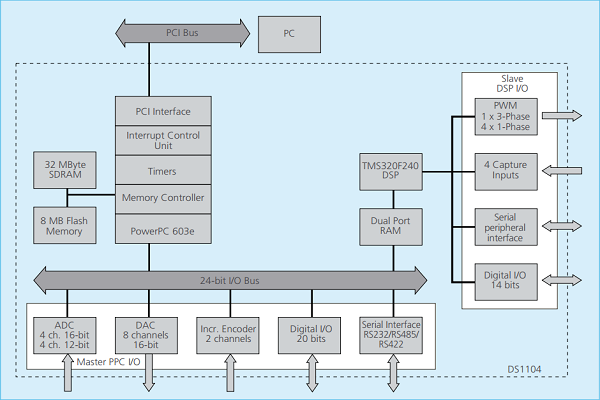
\includegraphics[width=1\textwidth]{DS1104 ControlBoard}
    \caption{DS1104 architecture}
    \label{fig:Fig1}
    \end{minipage}
    \hfill
    \centering
    \begin{minipage}{0.49\textwidth}
    \centering
    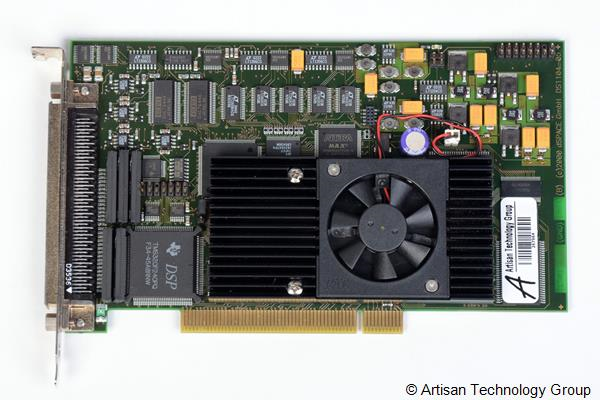
\includegraphics[width=1\textwidth]{Images/Upper_View}
    \caption{DS1104 Control Board}
    \label{fig:Fig2}
    \end{minipage}
\end{figure}

\subsubsection{Connection to External Devices}
There are three different ways to connect external devices to the DS1104. To access the I/O units of the master PPC and the slave DSP, connect external devices
\begin{itemize}
    \item to the 100-pin I/O connector P1 of the DS1104, or
    \item to the adapter cable with two 50-pin Sub-D connectors P1A and P1B, that are included in the DS1104 hardware package, or
    \item to the optional connector panel CP1104 or the optional combined connector/LED panel CLP1104, which provides an additional array of LEDs indicating the states of the digital signals.
\end{itemize}
\subsubsection{Memory Features}
The DS1104 is equipped with two memory sections:
\begin{itemize}
    \item Global memory
    \subitem 32-MByte synchronous DRAM (SDRAM) for applications and data.
    \subitem Fully cached (L1 cache).
    \item Flash memory
    \subitem 8 MByte, divided into 4 blocks of 2 MByte each.
    \subitem 6.5 MByte can be used for a user-specific application.
    \subitem 1.5 MByte are reserved for the boot firmware.
    \subitem 8-bit read / write access by master PPC.
    \subitem At least 100,000 erase cycles possible.
\end{itemize}

\subsubsection{Timer Features}
The DS1104 board is equipped with 6 timer devices. The timers are driven by the bus clock, whose frequency is referred to as BCLK.\\
Using ControlDesk Next Generation, you can get the current BCLK value via the Properties controlbar.\\
The timers have the following characteristics:
\begin{itemize}
    \item Time Base Counter
    \subitem Free-running 64-bit up counter driven by BCLK/4
    \subitem Used for measurement of relative and absolute times
    \subitem Used for time-stamping
    \item Timers 0 … 3
    \subitem 32-bit down counters driven by BCLK/8
    \subitem Used as trigger source for periodic tasks
    \subitem When the counter reaches 0, the timer generates an interrupt and the counter is reloaded with the value of the period register.
    \item Decrementer
    \subitem 32-bit down counter driven by BCLK/4
    \subitem Used as trigger source for periodic tasks
    \subitem When the counter reaches 0 the timer generates an interrupt. A new counter value is set by software in the timer interrupt service routine.
\end{itemize}

\subsubsection{Timer names}
The names of the timers listed above are the names of the hardware timer devices used by RTLib. They differ from the names used by RTI Timer Interrupt block:\\

\begin{table}[!h]
    \centering
        \begin{tabularx}{\textwidth}{ 
        | >{\raggedright\arraybackslash}X 
        | >{\raggedright\arraybackslash}X |}
        \hline
        \rowcolor[HTML]{34CDF9}\textbf{Timer Device Name Used by RTLib} & \textbf{Timer Interrupt Name Used by RTI} \\
        \hline
        Timer 0  & Timer A interrupt \\
        Timer 1  & Timer B interrupt \\
        Timer 2  & -(not supported by RTI) \\
        Timer 3  & -(not supported by RTI) \\
        Decrementer  & Timer C interrupt \\
        \hline
        \end{tabularx}
    \caption{dSPACE Timers}
    \label{TimerNames}
\end{table}

\subsubsection {Timer interrupts for periodic events}
Timers 0 … 3 and the Decrementer provide timer interrupts that you can use to trigger periodic events in a real-time application. These 32-bit down counters generate an interrupt whenever they reach 0. Then the timer is automatically reloaded.

\subsubsection{Host Interface}
The DS1104 provides a PCI interface requiring a single 5 V PCI slot. The interface has the following characteristics:
\begin{itemize}
    \item Access from/to the host PC via 33 MHz-PCI interface.\newline
    The interface serves the board setup, program downloads and runtime data transfers from/to the host PC.
    \item Interrupt line\newline
The host interface provides a bidirectional interrupt line: Via this line, the host PC can send interrupt requests to the master PPC and vice versa. Both the host PC and the master PPC can monitor the state of the interrupt line to detect when the corresponding interrupt service is finished.
\end{itemize}
\subsection{Features Provided by the Master PPC}
The DS1104’s main processing unit, MPC8240, consists of:

\begin{itemize}
    \item A PowerPC 603e microprocessor (master PPC) on which the control models will be implemented.
    \subitem Running at 250 MHz (CPU clock)
    \subitem Containing a 16-KByte L1 data cache
    \subitem Containing a 16-KByte L1 instruction cache
    \item An interrupt controller
    \item A synchronous DRAM controller
    \item Several timers
    \item A PCI interface (5 V, 32 bit, 33 MHz)
\end{itemize}

The master PPC controls the following I/O features of the DS1104:

\begin{itemize}
    \item ADC Unit
    \item DAC Unit
    \item Bit I/O Unit
    \item Incremental Encoder Interface
    \item Serial Interface
\end{itemize}

\subsubsection{ADC Unit}
The master PPC on the DS1104 controls an ADC unit featuring two
different types of A/D converters:
\begin{itemize}
    \item 1 A/D converter (ADC1) multiplexed to four channels (signals ADCH1 … ADCH4).The input signals of the converter are selected by a 4:1 input multiplexer. The A/D converters have the following characteristics:
    \subitem 16-bit resolution
    \subitem ±10 V input voltage range
    \subitem ± 5 mV offset error
    \subitem ± 0.25 \% gain error
    \subitem > 80 dB (at 10 kHz) signal-to-noise ratio (SNR)
    \item 4 parallel A/D converters (ADC2 … ADC5) with one channel each (signals ADCH5 … ADCH8). The A/D converters have the following characteristics:
    \subitem 12-bit resolution
    \subitem ±10 V input voltage range
    \subitem ± 5 mV offset error
    \subitem ± 0.5 \% gain error
    \subitem > 70 dB signal-to-noise ratio (SNR)
\end{itemize}
\textbf{Read modes}\par
The A/D converters can be used in polling and in non-polling mode. In polling mode, the conversion values can be read if the end-of conversion flag in the ADC control register is set to 1. In non-polling mode, the conversion values are read immediately without waiting on the completion of the conversion. The non-polling functions are \textit{ds1104\_adc\_read\_ch\_immediately} and \textit{ds1104\_adc\_read\_conv\_immediately}.

\noindent \textbf{Signal mapping}\par

\renewcommand{\arraystretch}{1.35}
\begin{table}[!h]
\begin{adjustbox}{width=1\textwidth}
\small
\begin{tabular}{|llllllll|}
\hline
\rowcolor[HTML]{34CDF9} 
\multicolumn{1}{|l|}{\cellcolor[HTML]{34CDF9}{\color[HTML]{333333} }} &
  \multicolumn{4}{l|}{\cellcolor[HTML]{34CDF9}{\color[HTML]{333333} \textbf{Channel/Bit Numbers of Related RTI Blocks/RTLib Functions}}} &
  \multicolumn{3}{l|}{\cellcolor[HTML]{34CDF9}{\color[HTML]{333333} \textbf{I/O Pin on …}}} \\ \cline{2-8} 
\rowcolor[HTML]{34CDF9} 
\multicolumn{1}{|l|}{\multirow[t]{-2}{*}{\cellcolor[HTML]{34CDF9}{\color[HTML]{333333} \textbf{Signal}}}} &
  \multicolumn{1}{l|}{\cellcolor[HTML]{34CDF9}{\color[HTML]{333333} \textbf{Related RTI Block(s)}}} &
  \multicolumn{1}{l|}{\cellcolor[HTML]{34CDF9}{\color[HTML]{333333} \textbf{Ch/Bit (RTI)}}} &
  \multicolumn{1}{l|}{\cellcolor[HTML]{34CDF9}{\color[HTML]{333333} \textbf{Related RTLib Functions}}} &
  \multicolumn{1}{l|}{\cellcolor[HTML]{34CDF9}{\color[HTML]{333333} \textbf{Ch/Bit (RTILib)}}} &
  \multicolumn{1}{l|}{\cellcolor[HTML]{34CDF9}{\color[HTML]{333333} \textbf{DS1104}}} &
  \multicolumn{1}{l|}{\cellcolor[HTML]{34CDF9}{\color[HTML]{333333} \textbf{Sub-D Conn.}}} &
  {\color[HTML]{333333} \textbf{CP/CLP}} \\ \hline
\multicolumn{8}{|l|}{\textbf{ADC Unit}} \\ \hline
\multicolumn{8}{|l|}{} \\
\multicolumn{8}{|l|}{} \\
\multicolumn{8}{|l|}{\multirow{-3}{*}{\begin{tabular}[c]{@{}l@{}}\tabitem Imput voltage range: ± 10 V\\ \tabitem ADCH1 ... ADCH4: input for A/D converter with 16-bit resolution\\ \tabitem ADCH5 ... ADCH8: input for A/D converter with 12-bit resolution\end{tabular}}} \\
\multicolumn{1}{|l|}{ADCH1} &
  \multicolumn{1}{l|}{} &
  \multicolumn{1}{l|}{Ch 1} &
  \multicolumn{1}{l|}{} &
  \multicolumn{1}{l|}{Ch 1} &
  \multicolumn{1}{l|}{P1 100} &
  \multicolumn{1}{l|}{P1A 50} &
  CP1 \\
\multicolumn{1}{|l|}{ADCH2} &
  \multicolumn{1}{l|}{} &
  \multicolumn{1}{l|}{Ch 2} &
  \multicolumn{1}{l|}{} &
  \multicolumn{1}{l|}{Ch 2} &
  \multicolumn{1}{l|}{P1 99} &
  \multicolumn{1}{l|}{P1B 50} &
  CP2 \\
\multicolumn{1}{|l|}{ADCH3} &
  \multicolumn{1}{l|}{} &
  \multicolumn{1}{l|}{Ch 3} &
  \multicolumn{1}{l|}{} &
  \multicolumn{1}{l|}{Ch 3} &
  \multicolumn{1}{l|}{P1 96} &
  \multicolumn{1}{l|}{P1A 33} &
  CP3 \\
\multicolumn{1}{|l|}{ADCH4} &
  \multicolumn{1}{l|}{\multirow[t]{-4}{*}{DS1104MUX\_ADC}} &
  \multicolumn{1}{l|}{Ch 4} &
  \multicolumn{1}{l|}{\multirow[t]{-4}{*}{See ADC Unit}} &
  \multicolumn{1}{l|}{Ch 4} &
  \multicolumn{1}{l|}{P1 95} &
  \multicolumn{1}{l|}{P1B 33} &
  CP4 \\
\multicolumn{1}{|l|}{ADCH5} &
  \multicolumn{1}{l|}{} &
  \multicolumn{1}{l|}{Ch 5} &
  \multicolumn{1}{l|}{} &
  \multicolumn{1}{l|}{Ch 5} &
  \multicolumn{1}{l|}{P1 92} &
  \multicolumn{1}{l|}{P1A 16} &
  CP5 \\
\multicolumn{1}{|l|}{ADCH6} &
  \multicolumn{1}{l|}{} &
  \multicolumn{1}{l|}{Ch 6} &
  \multicolumn{1}{l|}{} &
  \multicolumn{1}{l|}{Ch 6} &
  \multicolumn{1}{l|}{P1 91} &
  \multicolumn{1}{l|}{P1B 16} &
  CP6 \\
\multicolumn{1}{|l|}{ADCH7} &
  \multicolumn{1}{l|}{} &
  \multicolumn{1}{l|}{Ch 7} &
  \multicolumn{1}{l|}{} &
  \multicolumn{1}{l|}{Ch 7} &
  \multicolumn{1}{l|}{P1 88} &
  \multicolumn{1}{l|}{P1A 48} &
  CP7 \\
\multicolumn{1}{|l|}{ADCH8} &
  \multicolumn{1}{l|}{\multirow[t]{-4}{*}{DS1104ADC\_Cx}} &
  \multicolumn{1}{l|}{Ch 8} &
  \multicolumn{1}{l|}{\multirow[t]{-4}{*}{See ADC Unit}} &
  \multicolumn{1}{l|}{Ch 8} &
  \multicolumn{1}{l|}{P1 87} &
  \multicolumn{1}{l|}{P1B 48} &
  CP8 \\ \hline
\end{tabular}
\end{adjustbox}
\caption{ADC Signal mapping }
\label{ADC SignalMapping}
\end{table}

\noindent \textbf{Input circuit}\par
The following illustration is a simplified diagram of the input circuitry of the ADCs.
\begin{figure}[H]
    \centering
    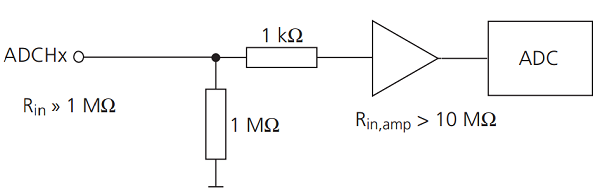
\includegraphics[width=0.75\textwidth]{Images/ADCs.png}
    \caption{ADCs Input Circuit}
    \label{ADCs}
\end{figure}
\ \\
\noindent \textbf{RTI/RTLib support}\par
You can access the master PPC’s ADC unit via RTI1104 and RTLib1104.\\
For details, see:
\begin{itemize}
    \item ADC Unit in the DS1104 RTI Reference
    \item ADC Unit in the DS1104 RTLib Reference
\end{itemize}

\noindent \textbf{DS1104MUX\_ADC}\par
The purpose of this block is to read up to four channels of the A/D Converter specifying the channels to be multiplexed. The width of the block output vector (comprising the selected channels assigned to one converter) matches the number of the selected channels.\par
\begin{figure}[H]
    \centering
    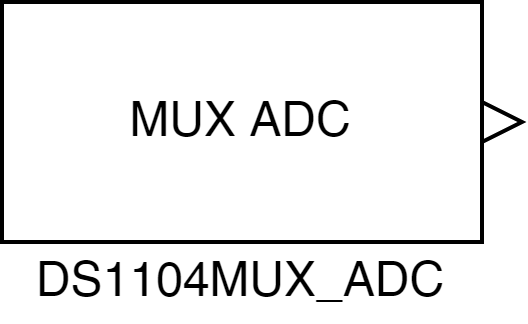
\includegraphics[width=0.25\textwidth]{Images/DS1104MUX_ADC.png}
    \caption{MUX ADC Block}
    \label{MUX ADC}
\end{figure}

\noindent \textbf{DS1104ADC\_Cx}\par
The purpose of this block is to read from a single channel of one of 4 parallel A/D converter channels. Lets you select a single channel within the range 5 … 8 and it´s scales between the analog input voltage and the output of the block:
\begin{table}[H]
    \centering
        \begin{tabularx}{0.6\textwidth}{ 
        | >{\raggedright\arraybackslash}X 
        | >{\raggedright\arraybackslash}X |}
        \hline
        \rowcolor[HTML]{34CDF9}\textbf{Input Voltage Range} & \textbf{Simulink Output} \\
        \hline
        –10 V ... +10 V  & –1 ... +1 (double) \\
        \hline
        \end{tabularx}
    \caption{ADC I/O characteristics}
    \label{ADC I/O characteristics}
\end{table}
\begin{figure}[H]
    \centering
    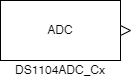
\includegraphics[width=0.25\textwidth]{Images/DS1104ADC_Cx.png}
    \caption{ADC\_Cx Block}
    \label{ADC_Cx}
\end{figure}

\subsubsection{DAC Unit}
The master PPC on the DS1104 controls a D/A converter. It has the following characteristics:
\begin{itemize}
    \item 8 parallel DAC channels (signals DACH1 … DACH8)
    \item 16-bit resolution
    \item ± 10 V output voltage range
    \item ± 1 mV offset error, 10 $\mu$V/K offset drift
    \item ± 0.1\% gain error, 25 ppm/K gain drift
    \item > 80 dB (at 10 kHz) signal-to-noise ratio (SNR)
    \item Transparent and latched mode
\end{itemize}
\textbf{Transparent and latched mode}\par
The DAC unit of the master PPC can be driven in two operating modes:
\begin{itemize}
    \item In the \textit{transparent mode}, the converted value is output immediately.
    \item In the \textit{latched mode}, the converted value is output after a strobe signal. This allows you to write output values to more than one channel, and output the values simultaneously.
\end{itemize}

\noindent \textbf{Synchronization with ST1PWM signal}\par
Updating DAC outputs can be synchronized with PWM signal generation or an external trigger source. 

\noindent \textbf{I/O - signal mapping}\par
The following table shows the mapping between the RTI block and RTLib functions and the corresponding pins used by the DAC unit.

\renewcommand{\arraystretch}{1.15}
\begin{table}[H]
\begin{adjustbox}{width=1\textwidth}
\small
\begin{tabular}{|llllllll|}
\hline
\rowcolor[HTML]{34CDF9} 
\multicolumn{1}{|l|}{\cellcolor[HTML]{34CDF9}{\color[HTML]{333333} }} &
  \multicolumn{4}{l|}{\cellcolor[HTML]{34CDF9}{\color[HTML]{333333} \textbf{Channel/Bit Numbers of Related RTI Blocks/RTLib Functions}}} &
  \multicolumn{3}{l|}{\cellcolor[HTML]{34CDF9}{\color[HTML]{333333} \textbf{I/O Pin on …}}} \\ \cline{2-8} 
\rowcolor[HTML]{34CDF9} 
\multicolumn{1}{|l|}{\multirow[t]{-2}{*}{\cellcolor[HTML]{34CDF9}{\color[HTML]{333333} \textbf{Signal}}}} &
  \multicolumn{1}{l|}{\cellcolor[HTML]{34CDF9}{\color[HTML]{333333} \textbf{Related RTI Block(s)}}} &
  \multicolumn{1}{l|}{\cellcolor[HTML]{34CDF9}{\color[HTML]{333333} \textbf{Ch/Bit (RTI)}}} &
  \multicolumn{1}{l|}{\cellcolor[HTML]{34CDF9}{\color[HTML]{333333} \textbf{Related RTLib Functions}}} &
  \multicolumn{1}{l|}{\cellcolor[HTML]{34CDF9}{\color[HTML]{333333} \textbf{Ch/Bit (RTILib)}}} &
  \multicolumn{1}{l|}{\cellcolor[HTML]{34CDF9}{\color[HTML]{333333} \textbf{DS1104}}} &
  \multicolumn{1}{l|}{\cellcolor[HTML]{34CDF9}{\color[HTML]{333333} \textbf{Sub-D Conn.}}} &
  {\color[HTML]{333333} \textbf{CP/CLP}} \\ \hline
\multicolumn{8}{|l|}{\textbf{DAC Unit}} \\ \hline
\multicolumn{8}{|l|}{} \\
\multicolumn{8}{|l|}{} \\
\multicolumn{8}{|l|}{\multirow{-3}{*}{\begin{tabular}[c]{@{}l@{}}\tabitem Output voltage range: ± 10 V\\ 
\tabitem Output current range: ± 5 mA\\
\tabitem DACH1 ... DACH8: D/A converter output with 16-bit resolution\\ 
\end{tabular}}} \\
\multicolumn{1}{|l|}{DACH1} &
  \multicolumn{1}{l|}{} &
  \multicolumn{1}{l|}{Ch 1} &
  \multicolumn{1}{l|}{} &
  \multicolumn{1}{l|}{Ch 1} &
  \multicolumn{1}{l|}{P1 84} &
  \multicolumn{1}{l|}{P1A 31} &
  CP9 \\
\multicolumn{1}{|l|}{DACH2} &
  \multicolumn{1}{l|}{} &
  \multicolumn{1}{l|}{Ch 2} &
  \multicolumn{1}{l|}{} &
  \multicolumn{1}{l|}{Ch 2} &
  \multicolumn{1}{l|}{P1 83} &
  \multicolumn{1}{l|}{P1B 31} &
  CP10 \\
\multicolumn{1}{|l|}{DACH3} &
  \multicolumn{1}{l|}{} &
  \multicolumn{1}{l|}{Ch 3} &
  \multicolumn{1}{l|}{} &
  \multicolumn{1}{l|}{Ch 3} &
  \multicolumn{1}{l|}{P1 80} &
  \multicolumn{1}{l|}{P1A 14} &
  CP11 \\
\multicolumn{1}{|l|}{DACH4} &
  \multicolumn{1}{l|}{\multirow[t]{-4}{*}{DS1104DAC\_Cx}} &
  \multicolumn{1}{l|}{Ch 4} &
  \multicolumn{1}{l|}{} &
  \multicolumn{1}{l|}{Ch 4} &
  \multicolumn{1}{l|}{P1 79} &
  \multicolumn{1}{l|}{P1B 14} &
  CP12 \\
\multicolumn{1}{|l|}{DACH5} &
  \multicolumn{1}{l|}{} &
  \multicolumn{1}{l|}{Ch 5} &
  \multicolumn{1}{l|}{} &
  \multicolumn{1}{l|}{Ch 5} &
  \multicolumn{1}{l|}{P1 76} &
  \multicolumn{1}{l|}{P1A 46} &
  CP13 \\
\multicolumn{1}{|l|}{DACH6} &
  \multicolumn{1}{l|}{} &
  \multicolumn{1}{l|}{Ch 6} &
  \multicolumn{1}{l|}{} &
  \multicolumn{1}{l|}{Ch 6} &
  \multicolumn{1}{l|}{P1 75} &
  \multicolumn{1}{l|}{P1B 46} &
  CP14 \\
\multicolumn{1}{|l|}{DACH7} &
  \multicolumn{1}{l|}{} &
  \multicolumn{1}{l|}{Ch 7} &
  \multicolumn{1}{l|}{} &
  \multicolumn{1}{l|}{Ch 7} &
  \multicolumn{1}{l|}{P1 72} &
  \multicolumn{1}{l|}{P1A 29} &
  CP15 \\
\multicolumn{1}{|l|}{DACH8} &
  \multicolumn{1}{l|}{} &
  \multicolumn{1}{l|}{Ch 8} &
  \multicolumn{1}{l|}{\multirow[t]{-8}{*}{See DAC Unit}} &
  \multicolumn{1}{l|}{Ch 8} &
  \multicolumn{1}{l|}{P1 71} &
  \multicolumn{1}{l|}{P1B 29} &
  CP16 \\ \hline
\end{tabular}
\end{adjustbox}
\caption{DAC I/O - Signal mapping }
\label{DACSignalMapping}
\end{table}

\noindent \textbf{Output circuit}\par
The following illustration is a simplified diagram of the output circuitry of the DACs.
\begin{figure}[H]
    \centering
    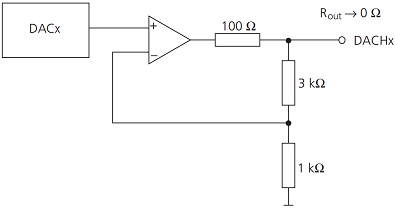
\includegraphics[width=0.75\textwidth]{Images/DACx.png}
    \caption{DACs Output Circuit}
    \label{DACs}
\end{figure}

\noindent \textbf{Electrical characteristics}\par
The analog outputs are single-ended bipolar outputs with the following characteristics.
\begin{table}[H]
\centering
\begin{tabular}{|l|ll|}
\hline
\rowcolor[HTML]{34CDF9} 
Parameter                   & \multicolumn{2}{l|}{\cellcolor[HTML]{34CDF9}Value} \\ \hline
                            & \multicolumn{1}{l|}{Min.}          & Max.          \\
Output voltage              & \multicolumn{1}{l|}{-10 V}         & +10 V         \\
Output current              & \multicolumn{1}{l|}{-5 mA}         & +5mA          \\ \hline
Output resistance           & \multicolumn{2}{l|}{$\rightarrow$ 0 $\Omega$}                         \\ \hline
Power-up default            & \multicolumn{2}{l|}{0 V}                           \\ \hline
SNR (signal-to-noise ratio) & \multicolumn{2}{l|}{\textgreater 80 dB}            \\ \hline
\end{tabular}
\caption{DAC Electrical output characteristics}
\end{table}

\noindent \textbf{RTI/RTLib support}\par
You can access the master PPC’s DAC unit via RTI1104 and RTLib1104 to write to one of the 8 parallel D/A converter channels.\\
\begin{figure}[H]
    \centering
    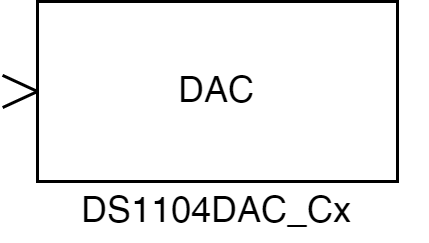
\includegraphics[width=0.25\textwidth]{Images/DS1104MUX_DAC.png}
    \caption{DAC\_Cx Block}
    \label{DAC_Cx}
\end{figure}

\noindent \textbf{I/O characteristics}\par
\begin{itemize}
    \item Scaling between the analog output voltage and the input of the block:
    \begin{table}[H]
    \centering
        \begin{tabularx}{0.6\textwidth}{ 
        | >{\raggedright\arraybackslash}X 
        | >{\raggedright\arraybackslash}X |}
        \hline
        \rowcolor[HTML]{34CDF9}\textbf{Simulink Input} & \textbf{Output Voltage Range} \\
        \hline
        –1 ... +1 (double)  & –10 V ... +10 V \\
        \hline
        \end{tabularx}
    \caption{DAC I/O characteristics}
    \label{DAC I/O characteristics}
\end{table}
    \item The block provides its outputs in:
    \subitem Transparent mode, that is the channel is converted and output immediately.
    \subitem Latched mode, that is the channel is converted after synchronous triggering.
\end{itemize}

\noindent \textbf{Initialization}\par
During the model initialization phase, an initial output voltage value is written to each D/A channel. This is especially useful if a channel is used within a triggered or enabled subsystem that is not executed right from the start of the simulation.

With the initialization value, the channel has a defined output during this simulation phase.

In other words, lets you specify the initial output voltage at the start of the simulation. The value must remain in the output voltage range ±10 V.

\noindent \textbf{Termination}\par
When the simulation terminates, the channel holds the last output value by default. You can specify a user-defined output value on termination, and use these settings to drive your external hardware into a safe final condition.

The specified termination values of I/O channels are set when the simulation executes its termination function by setting the simState variable to STOP. If the real‑time process is stopped by using ControlDesk's Stop RTP command, the processor resets immediately without executing termination functions. The current values of the I/O channels are kept and the specified termination values are not set.

Output on termination lets you either keep the current output voltage when the simulation terminates, or set the output to a specified value. The value must remain in the output voltage range ±10 V
%%%%%%%%%%%%%%%%%%%%%%%%%%%%%%%%%%%%%%%%%%%%%%%%%%%%%%%%%%%%%%%%%%%%%

\subsubsection{Bit I/O Unit}
The master PPC on the DS1104 controls a bit I/O unit with the following characteristics:
\begin{itemize}
    \item 20-bit digital I/O
    \item Direction selectable for each channel individually
    \item ±5 mA maximum output current
    \item TTL voltage range for input and output
    \item You can also use the bit I/O unit provided by the slave DSP, which contains 14-bit digital I/O.
\end{itemize}

\noindent \textbf{I/O characteristics}\par 
Relationship between the digital input and the output of the DS1104BIT\_IN\_Cx block:
\begin{table}[H]
    \centering
    \begin{tabular}{|l|ll|}
        \hline
        \rowcolor[HTML]{34CDF9} 
        \textbf{Digital Input (TTL)} & \multicolumn{2}{l|}{\cellcolor[HTML]{34CDF9}\textbf{Simulink Output}}                                 \\
        \rowcolor[HTML]{34CDF9} 
        \textbf{}                    & \multicolumn{1}{l|}{\cellcolor[HTML]{34CDF9}\textbf{Without Data Typing}} & \textbf{With Data Typing} \\ \hline
        High & \multicolumn{1}{l|}{1 (double)} & 1 (boolean) \\
        Low  & \multicolumn{1}{l|}{0 (double)} & 0 (boolean) \\ \hline
    \end{tabular}
\caption{I/O Input characteristics}
\label{I/O Input characteristics}
\end{table}

Relation between the digital output and the input of the DS1104BIT\_OUT\_Cx block:
\begin{table}[H]
    \centering
\begin{tabular}{|ll|l|}
\hline
\rowcolor[HTML]{34CDF9} 
\textbf{Simulink Output}                      & \textbf{}   & \cellcolor[HTML]{34CDF9}\textbf{Digital Output (TTL)} \\
\rowcolor[HTML]{34CDF9} 
\multicolumn{1}{|l|}{\cellcolor[HTML]{34CDF9}\textbf{Without Data Typing}} & \textbf{With Data Typing} & \cellcolor[HTML]{34CDF9}\textbf{} \\ \hline
\multicolumn{1}{|l|}{\textgreater 0 (double)} & 1 (boolean) & High                                                  \\
\multicolumn{1}{|l|}{$\leq$0 (double)}            & 0 (boolean) & Low                                                   \\ \hline
\end{tabular}
\caption{I/O Output characteristics}
\label{I/O Output characteristics}
\end{table}
\ \\
\ \\

\noindent \textbf{Description}\par

During the model initialization phase, an initial digital output value is written to each channel. This is especially useful if a channel is used within a triggered or enabled subsystem that is not executed right from the start of the simulation. With the initialization value, all channels have defined outputs during this simulation phase.

When the simulation terminates, all channels hold their last digital output values by default. You can specify a user-defined output value on termination, and use these settings to drive your external hardware into a safe final condition.

The specified termination values of I/O channels are set when the simulation executes its termination function by setting the simState variable to STOP. If you stop the real‑time application by using ControlDesk Next Generation's Stop RTP ( ControlDesk Next Generation Reference) command, the processor resets immediately without executing termination functions. The current values of the I/O channels are kept and the specified termination values are not set.

\noindent \textbf{RTI block support}\par
The master PPC library contains several blocks for programming the digital I/O unit.

\textit{To read from the digital I/O port}
\begin{itemize}
    \item Use DS1104BIT\_IN\_Cx to read certain bits of the digital I/O port. Lets you select a channel within the range 0 … 19 where as the channels 16 … 19 are multiplexed with 4 external interrupts.
\end{itemize}

\begin{figure}[H]
    \centering
    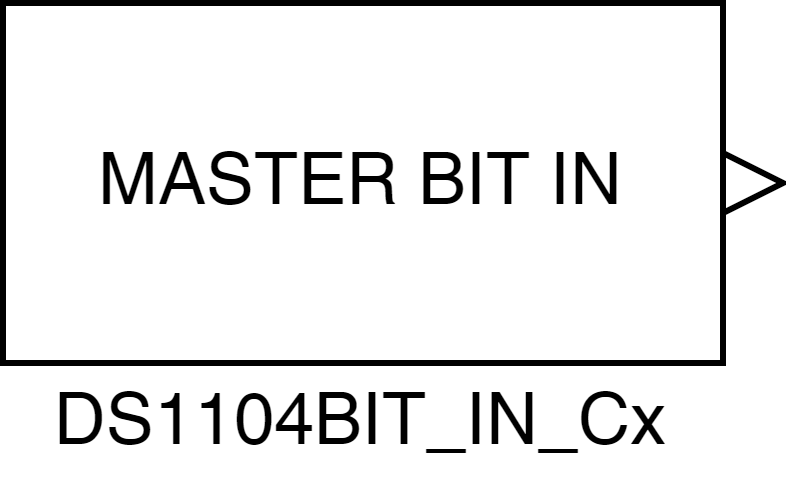
\includegraphics[width=0.35\textwidth]{Images/DS1104BIT_IN_Cx.png}
    \caption{BIT\_IN\_Cx Block}
    \label{BIT_IN_Cx}
\end{figure}

\textit{To write to the digital I/O port}
\begin{itemize}
    \item Use DS1104BIT\_OUT\_Cx to write certain bits of the digital I/O port.
\end{itemize}

\begin{figure}[H]
    \centering
    
\includegraphics[width=0.35\textwidth]{Images/MASTER BIT OUT.png}
    \caption{BIT\_OUT\_Cx Block}
    \label{BIT_OUT_Cx}
\end{figure}
\ \\
\ \\

The following table shows the mapping between the RTI blocks and RTLib functions and the corresponding pins used by the Bit I/O unit.

\begin{table}[H]
\begin{adjustbox}{width=1\textwidth}
\begin{tabular}{|lllllll|}
\hline
\multicolumn{1}{|l|}{\cellcolor[HTML]{34CDF9}\textbf{Signal}} &
  \multicolumn{3}{l|}{\cellcolor[HTML]{34CDF9}\textbf{Channel/Bit Numbers of Related RTI Blocks/RTLib Functions}} &
  \multicolumn{3}{l|}{\cellcolor[HTML]{34CDF9}\textbf{I/O Pin on …}} \\
\rowcolor[HTML]{34CDF9} 
\multicolumn{1}{|l|}{\cellcolor[HTML]{34CDF9}\textbf{}} &
  \multicolumn{1}{l|}{\cellcolor[HTML]{34CDF9}\textbf{Related RTI Blocks}} &
  \multicolumn{1}{l|}{\cellcolor[HTML]{34CDF9}\textbf{Ch/Bit (RTI)}} &
  \multicolumn{1}{l|}{\cellcolor[HTML]{34CDF9}\textbf{Ch/Bit (RTILib)}} &
  \multicolumn{1}{l|}{\cellcolor[HTML]{34CDF9}\textbf{DS1104}} &
  \multicolumn{1}{l|}{\cellcolor[HTML]{34CDF9}\textbf{CP/CLP}} &
  \textbf{Sub-D Conn.} \\ \hline
\rowcolor[HTML]{FFFFFF} 
\multicolumn{7}{|l|}{\cellcolor[HTML]{FFFFFF}\textbf{Bit I/O Unit}} \\ \hline
\multicolumn{7}{|l|}{\tabitem TTL voltage range} \\
\multicolumn{7}{|l|}{\tabitem Output current range: ±5 mA} \\
\multicolumn{1}{|l|}{IO0} &
  \multicolumn{1}{l|}{DS1104BIT\_IN\_Cx} &
  \multicolumn{1}{l|}{Bit 0} &
  \multicolumn{1}{l|}{Bit 0} &
  \multicolumn{1}{l|}{P1 68} &
  \multicolumn{1}{l|}{CP17 20} &
  P1A 12 \\
\multicolumn{1}{|l|}{IO1} &
  \multicolumn{1}{l|}{DS1104BIT\_OUT\_Cx} &
  \multicolumn{1}{l|}{Bit 1} &
  \multicolumn{1}{l|}{Bit 1} &
  \multicolumn{1}{l|}{P1 67} &
  \multicolumn{1}{l|}{CP17 2} &
  P1B 12 \\
\multicolumn{1}{|l|}{IO2} &
  \multicolumn{1}{l|}{} &
  \multicolumn{1}{l|}{Bit 2} &
  \multicolumn{1}{l|}{Bit 2} &
  \multicolumn{1}{l|}{P1 66} &
  \multicolumn{1}{l|}{CP17 21} &
  P1A 28 \\
\multicolumn{1}{|l|}{IO3} &
  \multicolumn{1}{l|}{} &
  \multicolumn{1}{l|}{Bit 3} &
  \multicolumn{1}{l|}{Bit 3} &
  \multicolumn{1}{l|}{P1 65} &
  \multicolumn{1}{l|}{CP17 3} &
  P1B 28 \\
\multicolumn{1}{|l|}{IO4} &
  \multicolumn{1}{l|}{} &
  \multicolumn{1}{l|}{Bit 4} &
  \multicolumn{1}{l|}{Bit 4} &
  \multicolumn{1}{l|}{P1 64} &
  \multicolumn{1}{l|}{CP17 23} &
  P1A 44 \\
\multicolumn{1}{|l|}{IO5} &
  \multicolumn{1}{l|}{} &
  \multicolumn{1}{l|}{Bit 5} &
  \multicolumn{1}{l|}{Bit 5} &
  \multicolumn{1}{l|}{P1 63} &
  \multicolumn{1}{l|}{CP17 5} &
  P1B 44 \\
\multicolumn{1}{|l|}{IO6} &
  \multicolumn{1}{l|}{} &
  \multicolumn{1}{l|}{Bit 6} &
  \multicolumn{1}{l|}{Bit 6} &
  \multicolumn{1}{l|}{P1 62} &
  \multicolumn{1}{l|}{CP17 24} &
  P1A 11 \\
\multicolumn{1}{|l|}{IO7} &
  \multicolumn{1}{l|}{} &
  \multicolumn{1}{l|}{Bit 7} &
  \multicolumn{1}{l|}{Bit 7} &
  \multicolumn{1}{l|}{P1 61} &
  \multicolumn{1}{l|}{CP17 6} &
  P1B 11 \\
\multicolumn{1}{|l|}{IO8} &
  \multicolumn{1}{l|}{} &
  \multicolumn{1}{l|}{Bit 8} &
  \multicolumn{1}{l|}{Bit 8} &
  \multicolumn{1}{l|}{P1 60} &
  \multicolumn{1}{l|}{CP17 26} &
  P1A 27 \\
\multicolumn{1}{|l|}{IO9} &
  \multicolumn{1}{l|}{} &
  \multicolumn{1}{l|}{Bit 9} &
  \multicolumn{1}{l|}{Bit 9} &
  \multicolumn{1}{l|}{P1 59} &
  \multicolumn{1}{l|}{CP17 8} &
  P1B 27 \\
\multicolumn{1}{|l|}{IO10} &
  \multicolumn{1}{l|}{} &
  \multicolumn{1}{l|}{Bit 10} &
  \multicolumn{1}{l|}{Bit 10} &
  \multicolumn{1}{l|}{P1 58} &
  \multicolumn{1}{l|}{CP17 27} &
  P1A 43 \\
\multicolumn{1}{|l|}{IO11} &
  \multicolumn{1}{l|}{} &
  \multicolumn{1}{l|}{Bit 11} &
  \multicolumn{1}{l|}{Bit 11} &
  \multicolumn{1}{l|}{P1 57} &
  \multicolumn{1}{l|}{CP17 9} &
  P1B 43 \\
\multicolumn{1}{|l|}{IO12} &
  \multicolumn{1}{l|}{} &
  \multicolumn{1}{l|}{Bit 12} &
  \multicolumn{1}{l|}{Bit 12} &
  \multicolumn{1}{l|}{P1 56} &
  \multicolumn{1}{l|}{CP17 29} &
  P1A 10 \\
\multicolumn{1}{|l|}{IO13} &
  \multicolumn{1}{l|}{} &
  \multicolumn{1}{l|}{Bit 13} &
  \multicolumn{1}{l|}{Bit 13} &
  \multicolumn{1}{l|}{P1 55} &
  \multicolumn{1}{l|}{CP17 11} &
  P1B 10 \\
\multicolumn{1}{|l|}{IO14} &
  \multicolumn{1}{l|}{} &
  \multicolumn{1}{l|}{Bit 14} &
  \multicolumn{1}{l|}{Bit 14} &
  \multicolumn{1}{l|}{P1 54} &
  \multicolumn{1}{l|}{CP17 30} &
  P1A 26 \\
\multicolumn{1}{|l|}{IO15} &
  \multicolumn{1}{l|}{} &
  \multicolumn{1}{l|}{Bit 15} &
  \multicolumn{1}{l|}{Bit 15} &
  \multicolumn{1}{l|}{P1 53} &
  \multicolumn{1}{l|}{CP17 12} &
  P1B 26 \\
\multicolumn{1}{|l|}{IO16} &
  \multicolumn{1}{l|}{} &
  \multicolumn{1}{l|}{Bit 16} &
  \multicolumn{1}{l|}{Bit 16} &
  \multicolumn{1}{l|}{P1 52} &
  \multicolumn{1}{l|}{CP17 32} &
  P1A 42 \\
\multicolumn{1}{|l|}{IO17} &
  \multicolumn{1}{l|}{} &
  \multicolumn{1}{l|}{Bit 17} &
  \multicolumn{1}{l|}{Bit 17} &
  \multicolumn{1}{l|}{P1 51} &
  \multicolumn{1}{l|}{CP17 14} &
  P1B 42 \\
\multicolumn{1}{|l|}{IO18} &
  \multicolumn{1}{l|}{} &
  \multicolumn{1}{l|}{Bit 18} &
  \multicolumn{1}{l|}{Bit 18} &
  \multicolumn{1}{l|}{P1 50} &
  \multicolumn{1}{l|}{CP17 33} &
  P1A 9 \\
\multicolumn{1}{|l|}{IO19} &
  \multicolumn{1}{l|}{} &
  \multicolumn{1}{l|}{Bit 19} &
  \multicolumn{1}{l|}{Bit 19} &
  \multicolumn{1}{l|}{P1 49} &
  \multicolumn{1}{l|}{CP17 15} &
  P1B 9 \\ \hline
\end{tabular}
\end{adjustbox}
\caption{Bit I/O Unit mapping}
\label{I/O Unit mapping}
\end{table}

\newpage

\section{Features Provided by the Slave DSP}
The DS1104’s slave DSP subsystem consists of
\begin{itemize}
    \item A Texas Instruments TMS320F240 DSP
    \subitem Running at 20 MHz
    \subitem 4Kx16 bit dual-port memory (DPMEM) used for communication with the master PPC
\end{itemize}

\subsection{Slave DSP Bit I/O Unit}
The slave DSP on the DS1104 provides a bit I/O unit with the following characteristics:
\begin{itemize}
    \item 14-bit digital I/O
    \item Direction selectable for each channel individually
    \item ±13 mA maximum output current
    \item TTL voltage range for input and output
\end{itemize}

\noindent \textbf{I/O mapping }\par

The following table shows the mapping between the RTI blocks and RTLib functions and the corresponding pins used by the slave DSP bit I/O unit.

\begin{table}[H]
\begin{adjustbox}{width=1\textwidth}
\small
\begin{tabular}{|lllllll|}
\hline
\rowcolor[HTML]{34CDF9} 
\multicolumn{1}{|l|}{\cellcolor[HTML]{34CDF9}\textbf{Signal}} &
  \multicolumn{3}{l|}{\cellcolor[HTML]{34CDF9}\textbf{Channel/Bit Numbers of Related RTI Blocks/RTLib Functions}} &
  \multicolumn{3}{l|}{\cellcolor[HTML]{34CDF9}\textbf{I/O Pin on …}} \\ \cline{5-7} 
\rowcolor[HTML]{34CDF9} 
\multicolumn{1}{|l|}{\cellcolor[HTML]{34CDF9}\textbf{}} &
  \multicolumn{1}{l|}{\cellcolor[HTML]{34CDF9}\textbf{Related RTI Block(s)}} &
  \multicolumn{1}{l|}{\cellcolor[HTML]{34CDF9}\textbf{Ch/Bit (RTI)}} &
  \multicolumn{1}{l|}{\cellcolor[HTML]{34CDF9}\textbf{Ch/Bit (RTILib)}} &
  \multicolumn{1}{l|}{\cellcolor[HTML]{34CDF9}\textbf{DS1104}} &
  \multicolumn{1}{l|}{\cellcolor[HTML]{34CDF9}\textbf{Sub-D Conn.}} &
  \textbf{CP/CLP} \\ \hline
\multicolumn{7}{|l|}{\textbf{Slave DSP Bit I/O Unit}} \\ \hline
\multicolumn{7}{|l|}{\tabitem TTL voltage range} \\
\multicolumn{7}{|l|}{\tabitem Output current range: ±13 mA} \\
\multicolumn{1}{|l|}{SPWM7 *} &
  \multicolumn{1}{l|}{DS1104SL\_DSP\_BIT\_IN\_Cx} &
  \multicolumn{1}{l|}{Bit 0} &
  \multicolumn{1}{l|}{Group 2 bit 0} &
  \multicolumn{1}{l|}{P1 31} &
  \multicolumn{1}{l|}{P1B 6} &
  CP18 10 \\
\multicolumn{1}{|l|}{SPWM8 *} &
  \multicolumn{1}{l|}{DS1104SL\_DSP\_BIT\_OUT\_Cx} &
  \multicolumn{1}{l|}{Bit 1} &
  \multicolumn{1}{l|}{Group 2 bit 1} &
  \multicolumn{1}{l|}{P1 29} &
  \multicolumn{1}{l|}{P1B 22} &
  CP18 29 \\
\multicolumn{1}{|l|}{SPWM9 *} &
  \multicolumn{1}{l|}{} &
  \multicolumn{1}{l|}{Bit 2} &
  \multicolumn{1}{l|}{Group 2 bit 2} &
  \multicolumn{1}{l|}{P1 27} &
  \multicolumn{1}{l|}{P1B 38} &
  CP18 11 \\
\multicolumn{1}{|l|}{ST1PWM *} &
  \multicolumn{1}{l|}{} &
  \multicolumn{1}{l|}{Bit 3} &
  \multicolumn{1}{l|}{Group 2 bit 3} &
  \multicolumn{1}{l|}{P1 25} &
  \multicolumn{1}{l|}{P1B 21} &
  CP18 23 \\
\multicolumn{1}{|l|}{ST2PWM *} &
  \multicolumn{1}{l|}{} &
  \multicolumn{1}{l|}{Bit 4} &
  \multicolumn{1}{l|}{Group 2 bit 4} &
  \multicolumn{1}{l|}{P1 23} &
  \multicolumn{1}{l|}{P1B 37} &
  CP18 5 \\
\multicolumn{1}{|l|}{ST3PWM *} &
  \multicolumn{1}{l|}{} &
  \multicolumn{1}{l|}{Bit 5} &
  \multicolumn{1}{l|}{Group 2 bit 5} &
  \multicolumn{1}{l|}{P1 21} &
  \multicolumn{1}{l|}{P1A 20} &
  CP18 24 \\
\multicolumn{1}{|l|}{SCAP1 *} &
  \multicolumn{1}{l|}{} &
  \multicolumn{1}{l|}{Bit 6} &
  \multicolumn{1}{l|}{Group 3 bit 4} &
  \multicolumn{1}{l|}{P1 18} &
  \multicolumn{1}{l|}{P1A 20} &
  CP18 2 \\
\multicolumn{1}{|l|}{SCAP2 *} &
  \multicolumn{1}{l|}{} &
  \multicolumn{1}{l|}{Bit 7} &
  \multicolumn{1}{l|}{Group 3 bit 5} &
  \multicolumn{1}{l|}{P1 16} &
  \multicolumn{1}{l|}{P1A 36} &
  CP18 21 \\
\multicolumn{1}{|l|}{SCAP3 *} &
  \multicolumn{1}{l|}{} &
  \multicolumn{1}{l|}{Bit 8} &
  \multicolumn{1}{l|}{Group 3 bit 6} &
  \multicolumn{1}{l|}{P1 14} &
  \multicolumn{1}{l|}{P1A 3} &
  CP18 3 \\
\multicolumn{1}{|l|}{SCAP4 *} &
  \multicolumn{1}{l|}{} &
  \multicolumn{1}{l|}{Bit 9} &
  \multicolumn{1}{l|}{Group 3 bit 7} &
  \multicolumn{1}{l|}{P1 12} &
  \multicolumn{1}{l|}{P1A 19} &
  CP18 22 \\
\multicolumn{1}{|l|}{SCLK *} &
  \multicolumn{1}{l|}{} &
  \multicolumn{1}{l|}{Bit 10} &
  \multicolumn{1}{l|}{Group 4 bit 0} &
  \multicolumn{1}{l|}{P1 17} &
  \multicolumn{1}{l|}{P1B 20} &
  CP18 17 \\
\multicolumn{1}{|l|}{SSTE *} &
  \multicolumn{1}{l|}{} &
  \multicolumn{1}{l|}{Bit 11} &
  \multicolumn{1}{l|}{Group 4 bit 1} &
  \multicolumn{1}{l|}{P1 15} &
  \multicolumn{1}{l|}{P1B 36} &
  CP18 35 \\
\multicolumn{1}{|l|}{SSIMO *} &
  \multicolumn{1}{l|}{} &
  \multicolumn{1}{l|}{Bit 12} &
  \multicolumn{1}{l|}{Group 4 bit 2} &
  \multicolumn{1}{l|}{P1 13} &
  \multicolumn{1}{l|}{P1B 3} &
  CP18 16 \\
\multicolumn{1}{|l|}{SSOMI *} &
  \multicolumn{1}{l|}{} &
  \multicolumn{1}{l|}{Bit 13} &
  \multicolumn{1}{l|}{Group 4 bit 3} &
  \multicolumn{1}{l|}{P1 11} &
  \multicolumn{1}{l|}{P1B 19} &
  CP18 34 \\ \hline
\end{tabular}
\end{adjustbox}
\caption{Slave DSP Bit I/O Unit}
\label{Slave DSP Bit I/O Unit}
\end{table}

\subsection{Slave DSP Timing I/O Unit}

The slave DSP on the DS1104 provides a timing I/O unit that you can use to generate and measure pulse-width modulated (PWM) and square-wave signals.

\noindent \textbf{PWM signal generation}\par

The PWM signal generation has the following characteristics:
\begin{itemize}
    \item Outputs for the generation of up to four 1-phase PWM signals with variable:
    \subitem Duty cycles (T/Tp ratio)
    \subitem PWM frequencies
    \subitem Polarity
    \subitem Symmetric or asymmetric PWM mode
    \item Non-inverted and inverted outputs for 3-phase PWM signal generation (PWM3) with variable:
    \subitem Duty cycles (T/Tp ratio)
    \subitem PWM frequencies
    \subitem Deadband
    \item Non-inverted and inverted outputs for the generation of 3-phase space vector PWM signals (PWMSV) with variable:
    \subitem Values T$_1$ and T$_2$ of the space vector
    \subitem Sector of the space vector
    \subitem PWM frequencies
    \subitem Deadband
\end{itemize}

\noindent \textbf{Square-wave signal generation (D2F)}\par

The square-wave signal generation (D2F) provides outputs for the generation of up to four square-wave signals with variable frequencies.

\noindent \textbf{PWM signal measurement (PWM2D)}\par

The PWM signal measurement (PWM2D) provides inputs for the measurement of the duty cycle and frequency of up to four PWM signals. For details, see Slave DSP PWM Signal Measurement (PWM2D) on page 60.

\noindent \textbf{Square-wave signal measurement (F2D)}\par

The square-wave signal measurement (F2D) provides inputs for the measurement of up to four square-wave signals.

\noindent \textbf{I/O mapping}\par
\begin{table}[H]
\begin{adjustbox}{width=1\textwidth}
\small
\begin{tabular}{|lllllll|}
\hline
\rowcolor[HTML]{34CDF9} 
\multicolumn{1}{|l|}{\cellcolor[HTML]{34CDF9}\textbf{Signal}} &
  \multicolumn{3}{l|}{\cellcolor[HTML]{34CDF9}\textbf{Channel/Bit Numbers of Related RTI Blocks/RTLib Functions}} &
  \multicolumn{3}{l|}{\cellcolor[HTML]{34CDF9}\textbf{I/O Pin on …}} \\ \cline{5-7} 
\rowcolor[HTML]{34CDF9} 
\multicolumn{1}{|l|}{\cellcolor[HTML]{34CDF9}\textbf{}} &
  \multicolumn{1}{l|}{\cellcolor[HTML]{34CDF9}\textbf{Related RTI Block(s)}} &
  \multicolumn{1}{l|}{\cellcolor[HTML]{34CDF9}\textbf{Ch/Bit (RTI)}} &
  \multicolumn{1}{l|}{\cellcolor[HTML]{34CDF9}\textbf{Ch/Bit (RTILib)}} &
  \multicolumn{1}{l|}{\cellcolor[HTML]{34CDF9}\textbf{DS1104}} &
  \multicolumn{1}{l|}{\cellcolor[HTML]{34CDF9}\textbf{Sub-D Conn.}} &
  \textbf{CP/CLP} \\ \hline
\multicolumn{7}{|l|}{\textbf{1‑Phase PWM Signal Generation (PWM), 3‑Phase PWM Signal Generation (PWM3), Space Vector PWM Signal Generation (PWMSV)}} \\ \hline
\multicolumn{7}{|l|}{TTL output voltage range} \\
\multicolumn{7}{|l|}{Output current range: ±13 mA} \\
\multicolumn{1}{|l|}{ST2PWM *} &
  \multicolumn{1}{l|}{DS1104SL\_DSP\_PWM} &
  \multicolumn{1}{l|}{Ch 1} &
  \multicolumn{1}{l|}{Ch 1} &
  \multicolumn{1}{l|}{P1 23} &
  \multicolumn{1}{l|}{P1B 21} &
  CP18 5 \\
\multicolumn{1}{|l|}{SPWM7 *} &
  \multicolumn{1}{l|}{DS1104SL\_DSP\_PWM3} &
  \multicolumn{1}{l|}{Ch 2} &
  \multicolumn{1}{l|}{Ch 2} &
  \multicolumn{1}{l|}{P1 31} &
  \multicolumn{1}{l|}{P1B 6} &
  CP18 10 \\
\multicolumn{1}{|l|}{SPWM8 *} &
  \multicolumn{1}{l|}{DS1104SL\_DSP\_PWMSV} &
  \multicolumn{1}{l|}{Ch 3} &
  \multicolumn{1}{l|}{Ch 3} &
  \multicolumn{1}{l|}{P1 29} &
  \multicolumn{1}{l|}{P1B 22} &
  CP18 29 \\
\multicolumn{1}{|l|}{SPWM9 *} &
  \multicolumn{1}{l|}{} &
  \multicolumn{1}{l|}{Ch 4} &
  \multicolumn{1}{l|}{Ch 4} &
  \multicolumn{1}{l|}{P1 27} &
  \multicolumn{1}{l|}{P1B 38} &
  CP18 11 \\
\multicolumn{1}{|l|}{SPWM1 *} &
  \multicolumn{1}{l|}{} &
  \multicolumn{1}{l|}{Phase 1} &
  \multicolumn{1}{l|}{Phase 1} &
  \multicolumn{1}{l|}{P1 32} &
  \multicolumn{1}{l|}{P1A 6} &
  CP18 7 \\
\multicolumn{1}{|l|}{SPWM3 *} &
  \multicolumn{1}{l|}{} &
  \multicolumn{1}{l|}{Phase 2} &
  \multicolumn{1}{l|}{Phase 2} &
  \multicolumn{1}{l|}{P1 28} &
  \multicolumn{1}{l|}{P1A 38} &
  CP18 8 \\
\multicolumn{1}{|l|}{SPWM5 *} &
  \multicolumn{1}{l|}{} &
  \multicolumn{1}{l|}{Phase 3} &
  \multicolumn{1}{l|}{Phase 3} &
  \multicolumn{1}{l|}{P1 24} &
  \multicolumn{1}{l|}{P1A 21} &
  CP18 9 \\
\multicolumn{1}{|l|}{SPWM2} &
  \multicolumn{1}{l|}{} &
  \multicolumn{1}{l|}{Phase 1 (inverted)} &
  \multicolumn{1}{l|}{Phase 1 (inverted)} &
  \multicolumn{1}{l|}{P1 30} &
  \multicolumn{1}{l|}{P1A 22} &
  CP18 26 \\
\multicolumn{1}{|l|}{SPWM4} &
  \multicolumn{1}{l|}{} &
  \multicolumn{1}{l|}{Phase 2 (inverted)} &
  \multicolumn{1}{l|}{Phase 2 (inverted)} &
  \multicolumn{1}{l|}{P1 26} &
  \multicolumn{1}{l|}{P1A 5} &
  CP18 27 \\
\multicolumn{1}{|l|}{SPWM6} &
  \multicolumn{1}{l|}{} &
  \multicolumn{1}{l|}{Phase 3 (inverted)} &
  \multicolumn{1}{l|}{Phase 3 (inverted)} &
  \multicolumn{1}{l|}{P1 22} &
  \multicolumn{1}{l|}{P1A 37} &
  CP18 28 \\ \hline
\end{tabular}
\end{adjustbox}
\caption{Slave DSP PWM Signal}
\label{Slave DSP PWM Signal}
\end{table}

\subsection{Basics of Slave DSP PWM Signal Generation}

The slave DSP of the DS1104 provides outputs for PWM signal generation. Each PWM pulse is centered around the middle of the corresponding PWM period (symmetric PWM generation mode).

\noindent \textbf{PWM signals}\par

PWM signal generation is crucial to many motor and motion control applications. PWM signals are pulse trains with fixed frequency and magnitude and variable pulse width. There is one pulse of fixed magnitude in every PWM period.

However, the width of the pulses changes from period to period according to a modulating signal. When a PWM signal is applied to the gate of a power transistor, it causes the turn-on/turn-off intervals of the transistor to change from one PWM period to another, according to the same modulating signal. The frequency of a PWM signal is usually much higher than that of the modulating signal, or the fundamental frequency, so that the energy delivered to the motor and its load depends mainly on the modulating signal.

\noindent \textbf{PWM period, duty cycle and resolution}\par

For PWM signals, you can specify the PWM period TP (= T$_high$+ T$_low$) in the range 200 ns … 819,2 ms. For PWM3 and PWMSV signals, the PWM period TP applies to each of the 3 phases. For 1-phase PWM signals, the PWM period TP applies to each of the four PWM output channels. If you perform 3-phase and 1-phase PWM signal generation at the same time, you can specify different PWM periods for the 3-phase and 1-phase PWM signals.

You can also specify the duty cycle. The following illustration shows how the duty cycle d (= T$_high$/ TP) is defined. The available duty cycle range is 0 … 1 (0 … 100 \%).

\begin{figure}[H]
    \centering
    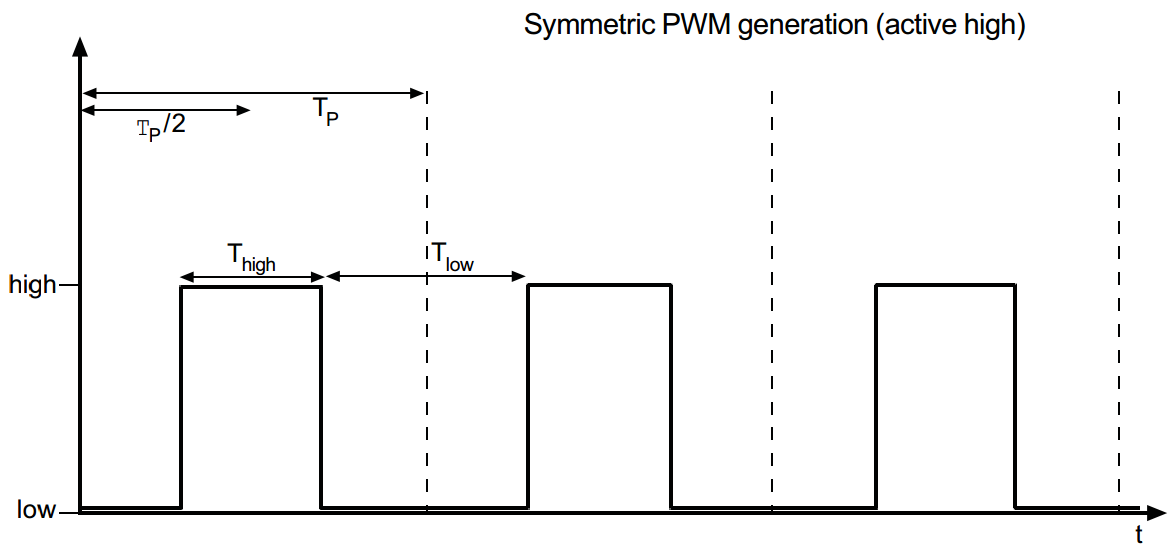
\includegraphics[width=\textwidth]{Images/Symmetric PWM generation.png}
    \caption{Symmetric PWM generation}
    \label{Symmetric PWM generation}
\end{figure}

Depending on the selected PWM period, the following resolutions are given. They apply to symmetric PWM signals.

\begin{table}[H]
\centering
\begin{tabular}{|l|l|}
\hline
\rowcolor[HTML]{34CDF9} 
\textbf{Period T$_p$} & \textbf{Resolution} \\ \hline
\textless 6.4 ms   & 100 ns              \\
\textless 12.8 ms  & 200 ns              \\
\textless 25.6 ms  & 400 ns              \\
\textless 51.2 ms  & 800 ns              \\
\textless 102.4 ms & 1.6 $\mu$s              \\
\textless 204.8 ms & 3.2 $\mu$s              \\
\textless 409.6 ms & 6.4 $\mu$s              \\
\textless 819.2 ms & 12.8 $\mu$s             \\ \hline
\end{tabular}
\caption{Symmetric PWM resolution}
%\label{Symmetric PWM resolution}
\end{table}

\noindent \textbf{Deadband}\par

For the three PWM duty cycles of PWM3 and PWMSV, you can specify one deadband value. This is the time gap between the rising and falling edges of the non-inverted and inverted PWM signals. The deadband introduces a time delay that allows complete turning off of one power transistor before the turning on of the other power transistor.

The maximum deadband value is 100 $\mu$s. However, it should not be greater than T$_P$/2.

\begin{figure}[H]
    \centering
    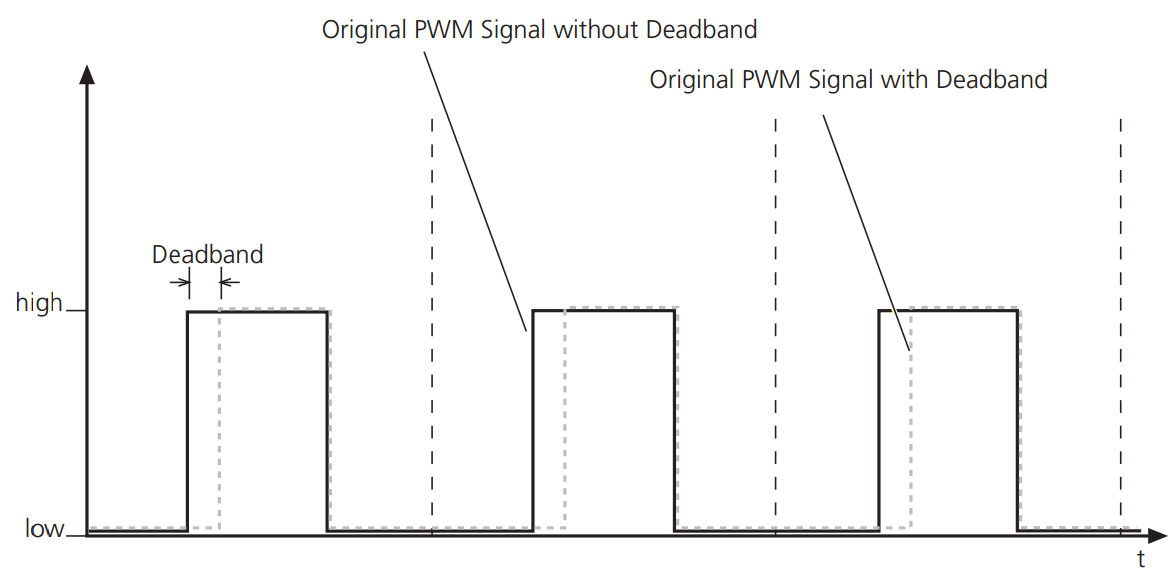
\includegraphics[width=\textwidth]{Images/Original PWM Signal with Deadband.png}
    \caption{Original PWM Signal with Deadband}
    \label{Original PWM Signal with Deadband}
\end{figure}

\begin{figure}[H]
    \centering
    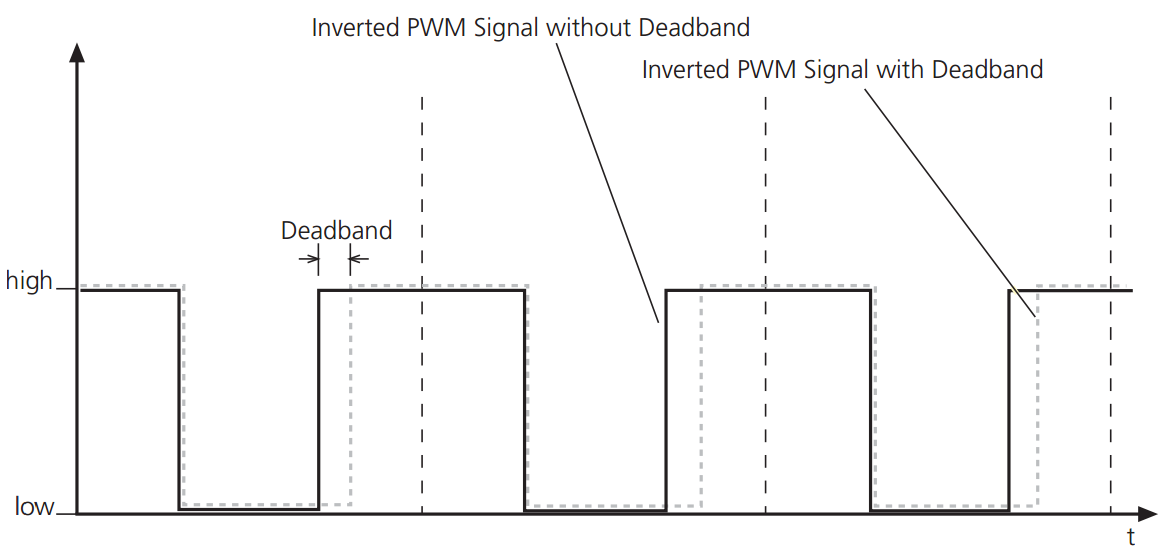
\includegraphics[width=\textwidth]{Images/Inverted PWM Signal with Deadband.png}
    \caption{Inverted PWM Signal with Deadband}
    \label{Inverted PWM Signal with Deadband}
\end{figure}

\noindent \textbf{PWM outputs}\par
For each of the PWM generation modes (1-phase, 3-phase and space vector), the PWM outputs can be specified. The running PWM generation can be suspended and the corresponding channels can be set to a specified TTL level (high or low). Only the output of the PWM signal is disabled. Signal calculation is still running and if you enable PWM generation, the currently calculated signal is output, and not the defined initialization or termination value. The PWM outputs can be specified for the two simulation phases (RTI):
\begin{itemize}
    \item During the initialization phase, you can disable the PWM generation of selected channels (channel pairs for PWM3 and PWMSV) and set each output (pair) to a defined TTL level (high or low). No signal is generated during the initialization.
    \item During run time, you can stop PWM generation and set the outputs to a defined TTL level (high or low). At any time you can resume in generating the PWM signal. If the simulation terminates the outputs can be set to defined TTL levels.
\end{itemize}

If the PWM stop feature is disabled, the normal initialization and termination routines are executed. That means the specified duty cycles for initialization and termination are used.

\subsection{1-Phase PWM Signal Generation (PWM)}

\noindent \textbf{Asymmetric PWM mode}
As an alternative to the symmetric PWM generation mode, you can also let each PWM pulse start at the beginning of the corresponding PWM period (asymmetric PWM mode). Switching between symmetric and asymmetric PWM mode applies to all of the four 1-phase PWM output channels. The following illustration shows two active high symmetric and asymmetric 1-phase PWM signals.
\begin{figure}[H]
    \centering
    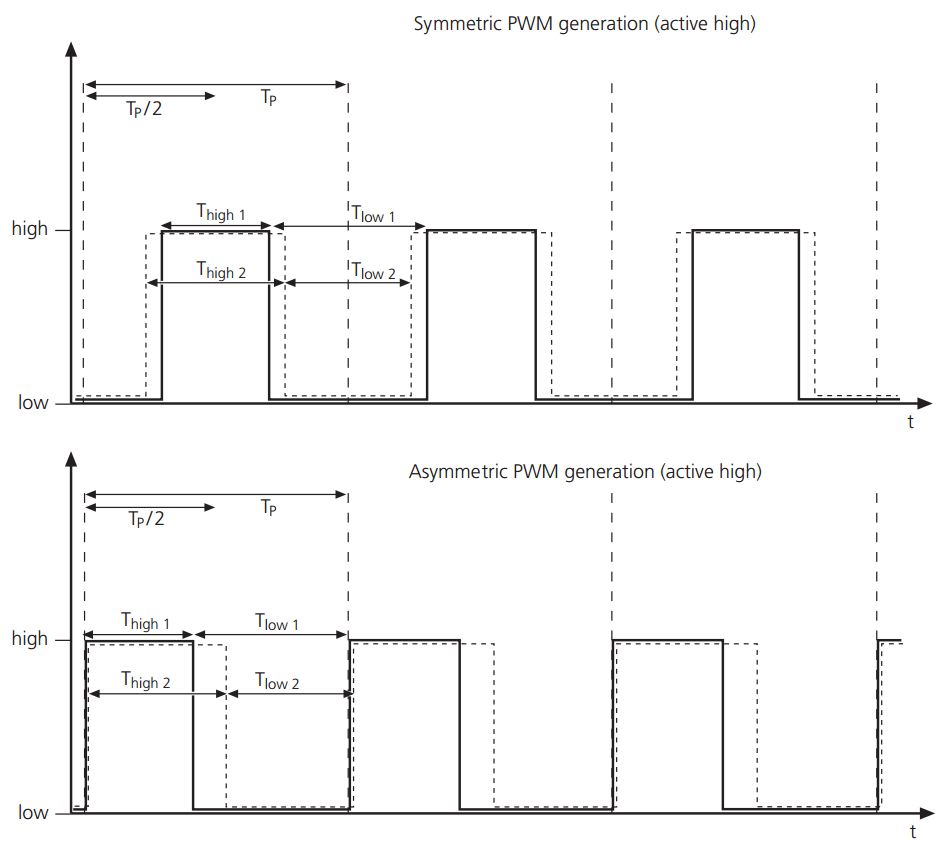
\includegraphics[width=\textwidth]{Images/Symmetric and asymmetric PWM generation.png}
    \caption{Symmetric and asymmetric PWM generation}
    \label{Symmetric and asymmetric PWM generation}
\end{figure}

\noindent \textbf{PWM period and resolution in asymmetric mode}\par

In the asymmetric mode, the PWM period T$_P$ must be in the range 200 ns … 409,6 ms. Depending on the period, the following resolutions are given:

\begin{table}[H]
\centering
\begin{tabular}{|l|l|}
\hline
\rowcolor[HTML]{34CDF9} 
\textbf{Period T$_p$} & \textbf{Resolution} \\ \hline
\textless 3.2 ms   & 50 ns              \\
\textless 6.4 ms   & 100 ns              \\
\textless 12.8 ms  & 200 ns              \\
\textless 25.6 ms  & 400 ns              \\
\textless 51.2 ms  & 800 ns              \\
\textless 102.4 ms & 1.6 $\mu$s              \\
\textless 204.8 ms & 3.2 $\mu$s              \\
\textless 409.6 ms & 6.4 $\mu$s              \\ \hline
\end{tabular}
\caption{Asymmetric PWM resolution}
%\label{Asymmetric PWM resolution}
\end{table}
\noindent \textit{Due to quantization effects, you will encounter considerable deviations between the desired PWM period T$_P$ and the generated PWM period, especially for higher PWM frequencies.}

\noindent \textbf{Polarity of PWM signals}\par

For each of the four 1-phase PWM channels, you can specify separately whether to generate active high or active low PWM signals.

\noindent \textbf{PWM output}\par
Via RTI you can specify separately for each of the four 1-phase PWM channels, whether or not to generate PWM signals. In case of PWM stop, the output of each channel can be set to TTL high or low.

\noindent \textbf{RTI/RTLib support}\par
You can perform 1-phase PWM signal generation on the slave DSP via RTI1104 and RTLib1104. For details, see
\begin{itemize}
    \item DS1104SL\_DSP\_PWM
    \item Slave DSP PWM Generation
\end{itemize}

Using the ST1PWM Pin

Objective
The ST1PWM pin is lead to the interrupt controller of the DS1104, so it is possible to generate interrupts that are synchronous to PWM signal generation. You can also use the pin as a further external interrupt input (user interrupt). In this case the ST1PWM pin has to be configured as an input (using RTLib1104).

Strobing I/O

In addition, you can use the ST1PWM pin for strobing the I/O (ADCs, DACs and incremental encoder signals). The required trigger signal can be either generated by the slave DSP or driven externally. In the second case the ST1PWM pin has to be configured as an input or the slave DSP must be in reset mode.

Recognizing signals at the ST1PWM pin

To allow the interrupt controller to recognize an incoming signal at the ST1PWM pin (PWM interrupt, external interrupt or trigger for strobing), the interrupt signal must be kept high for at least 1 $\mu$s. The interrupt is activated by the high to low transition of the signal. The signal must remain low for at least 100 ns after the transition.

\newpage 

\section{Hardware and software required for this project}

To implement a real-time control loop using dSPACE and MATLAB we need following items.

\begin{enumerate}
    \item dSPACE DS1104 R\&D Controller Board
        \begin{figure}[H]
            \centering
            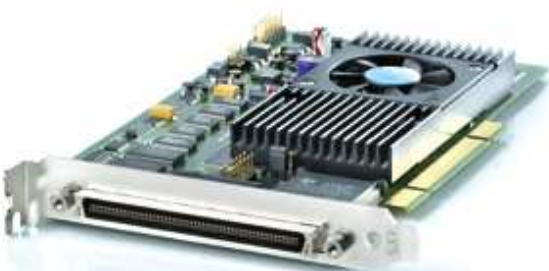
\includegraphics[width=0.4\textwidth]{Images/Ball and Bean/DS1104.png}
            \caption{Controller Board}
            \label{fig1}
        \end{figure}
    \item Dongle licenses on a USB flash disk
        \begin{figure}[H]
            \centering
            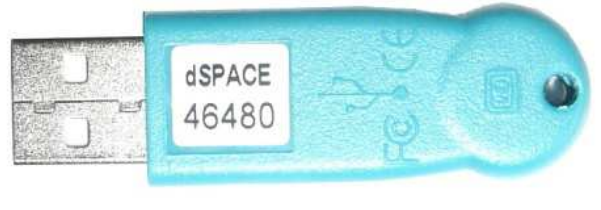
\includegraphics[width=0.25\textwidth]{Images/Ball and Bean/Dongle.png}
            \caption{Dongle USB flash}
            \label{fig2}
        \end{figure}
    \item Connector panel CLP1104
        \begin{figure}[H]
            \centering
            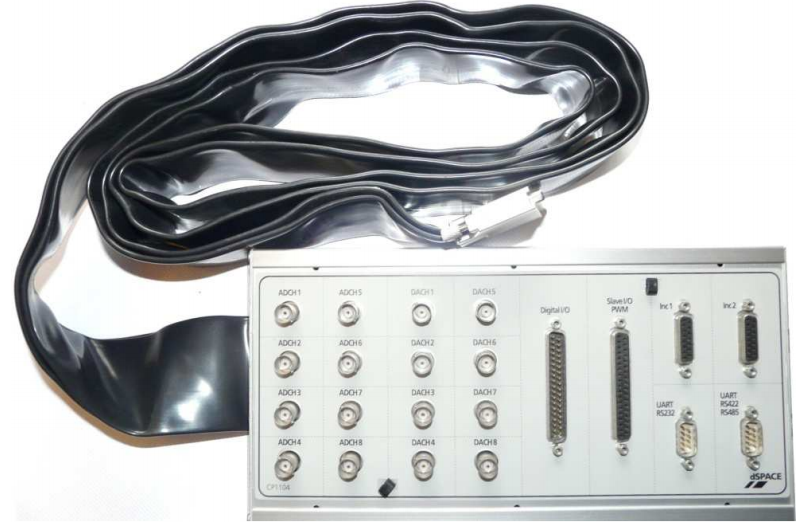
\includegraphics[width=0.5\textwidth]{Images/Ball and Bean/CLP1104.png}
            \caption{Connector panel}
            \label{fig3}
        \end{figure}
    \item D Sub 37 cable connector
        \begin{figure}[H]
            \centering
            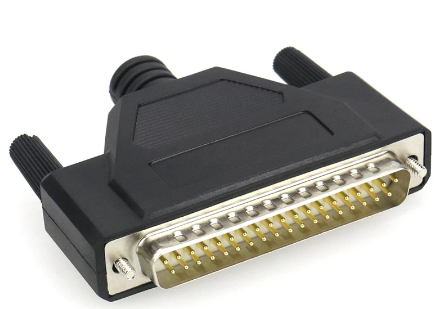
\includegraphics[width=0.35\textwidth]{Images/Ball and Bean/D-Sub37.png}
            \caption{Cable connector}
            \label{fig3.1}
        \end{figure}
    \item Servomotor Futaba S3003
        \begin{figure}[H]
            \centering
            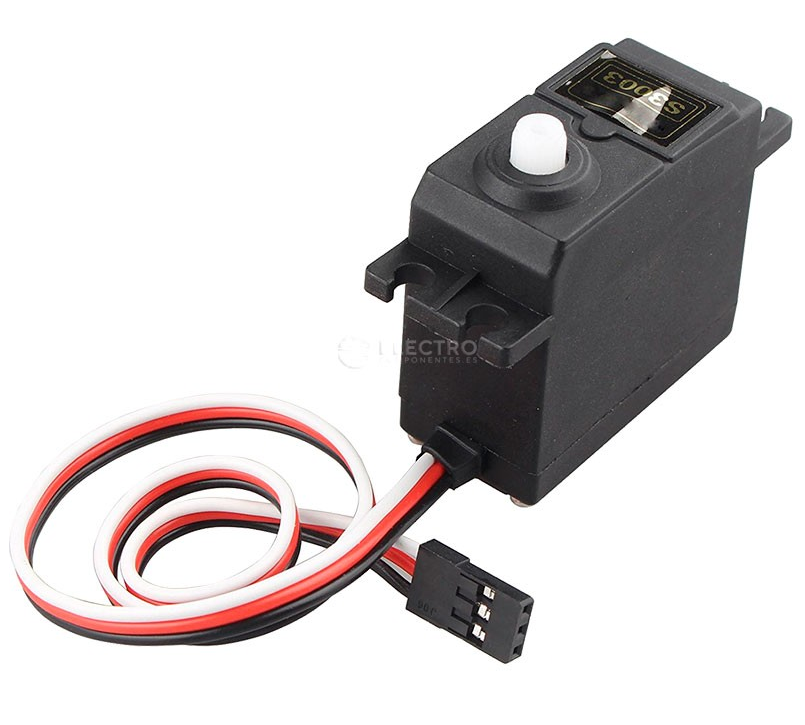
\includegraphics[width=0.4\textwidth]{Images/Ball and Bean/Servo.png}
            \caption{Futaba S3003}
            \label{fig3.2}
        \end{figure}
    \item Ultrasonic sensor HC-SR04
        \begin{figure}[H]
            \centering
            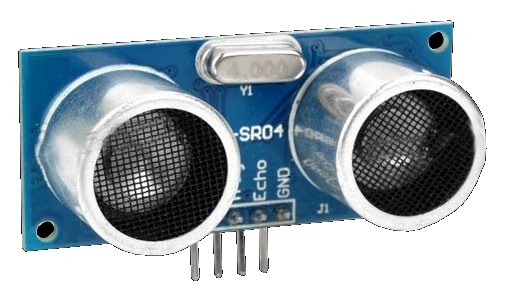
\includegraphics[width=0.4\textwidth]{Images/Ball and Bean/HC-SR04.png}
            \caption{HC-SR04}
            \label{fig3.3}
        \end{figure}
        
\end{enumerate}
\newpage

\section{Controller Design and Implementation in Simulink}
\subsection{Configuration of the Simulink model}
\begin{enumerate}
    
    \item The first step is start MATLAB and then, the following message appears, which says that dSPACE RealTime Interface (RTI) is installed for several hardware platforms, in this case, select DS1104.
    \begin{figure}[H]
        \centering
        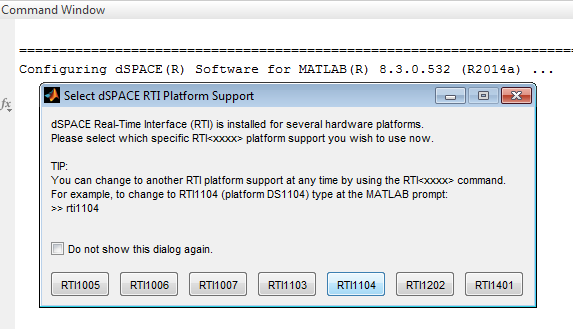
\includegraphics[width=0.7\textwidth]{Images/Ball and Bean/MatLab1.png}
        \caption{Selection of the RTI platform}
        \label{fig4}
    \end{figure}
By default, the workspace is placed in the user documents.
For a better organization of the generated files, change it to another directory because when you compile the Simulink model a \textbf{.sdf} file will be generated and without it, you won`t be able to work in the ControlDesk platform.
    
    
    \item  Some parameters must be adjusted before importing the model to ControlDesk. First, the solver and step time must be configured. To do so, click on the ‘Simulation’ button, and click on the option ‘Model Configuration Parameters’, which will open a new dialog window, as the one seen in figure \ref{fig6}. In ‘Solver Options’, select the type ‘Fixed-step’ and select the solver ‘ode4 (Runge-Kutta)’. In the option ‘Fixed-step size (fundamental sample time)’, a value must be entered such as it allows to have a good resolution of data capture, for this project, a value between 0.001 and 0.0001 is admissible.
    \begin{figure}[H]
        \centering
        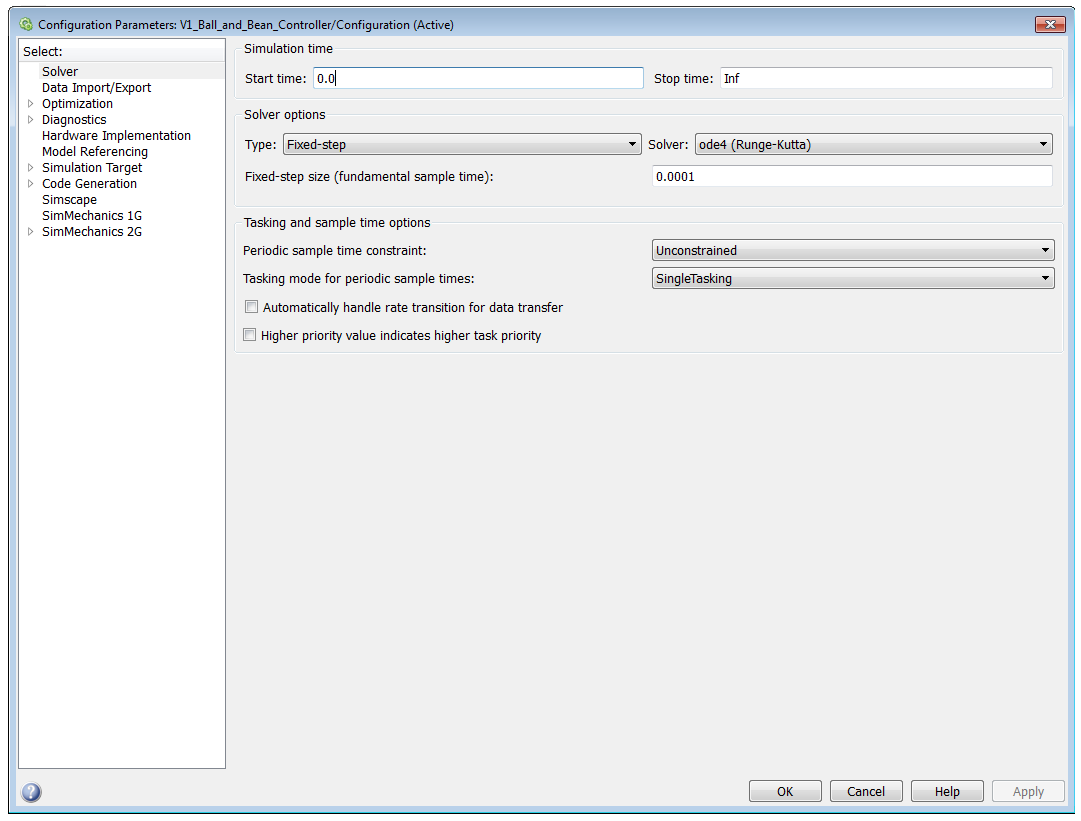
\includegraphics[width=0.7\textwidth]{Images/Ball and Bean/MatLab5.png}
        \caption{Configuration of integration step}
        \label{fig6}
    \end{figure}

    \item The option ‘Simulation Time’ must be set to ‘inf’. This can be done in the option ‘Solver’ of the ‘Model Configuration Parameters’ window, or in the box shown in the toolbar of Simulink, as seen in figure \ref{fig7}. This allows ControlDesk to simulate the model for an indefinite amount of time, instead of stopping the simulation at a specific time, as it is done normally in Simulink.
    \begin{figure}[H]
        \centering
        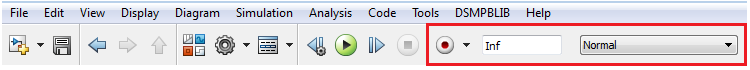
\includegraphics[width=0.7\textwidth]{Images/Ball and Bean/MatLab6.png}
        \caption{Change of simulation time to ‘Inf’}
        \label{fig7}
    \end{figure}

    \item The model must be saved as a .slx file in the main folder defined by the user in step 1.

    \item Finally, the model must be compiled in the dSPACE board. The DS1104 board must be selected in the ‘Model Configuration Parameters’ window, selecting the ‘Code Generation’ option, as seen in the figure \ref{fig8}. Press the button ‘Browse. . . ’ at the right of ‘System target file’ to open a window that will show a list of .tlc files, and select the one associated with the DS1104 board, as shown in figure \ref{fig9}.
    \begin{figure}[H]
        \centering
        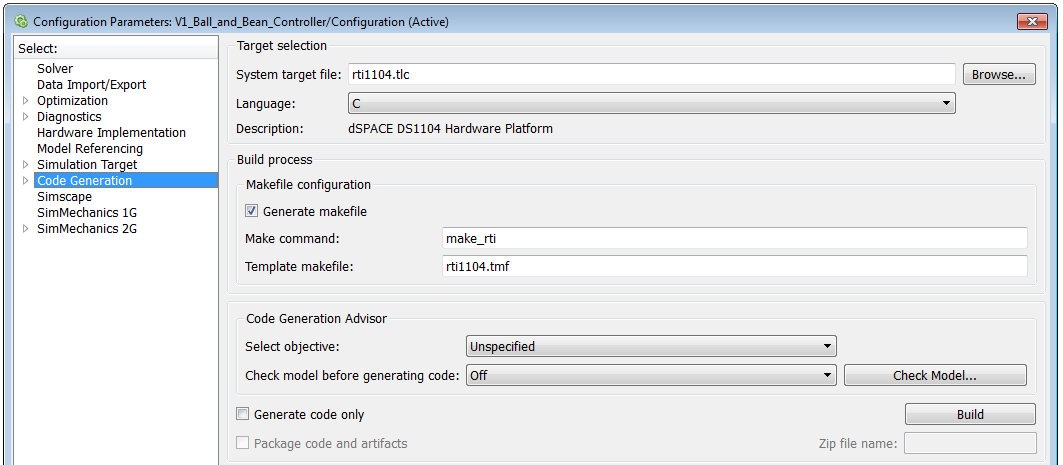
\includegraphics[width=0.7\textwidth]{Images/Ball and Bean/MatLab7.png}
        \caption{Selection of the board for compilation}
        \label{fig8}
    \end{figure}
    
    \begin{figure}[H]
        \centering
        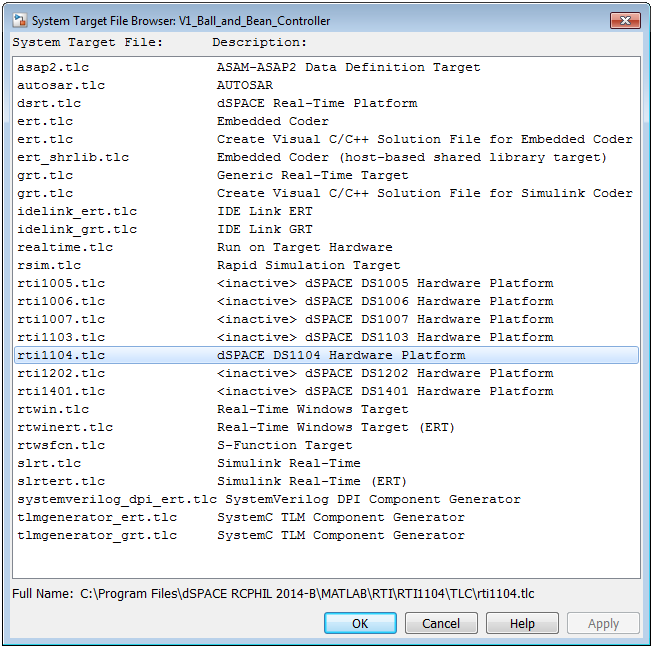
\includegraphics[width=0.7\textwidth]{Images/Ball and Bean/MatLab8.png}
        \caption{ Selection of the .tlc file related to the board}
        \label{fig9}
    \end{figure}

    \item The final step is to generate the code that will be compiled in the board. In Simulink, go to the menu ‘Code’, and in the option ‘C/C++ Code’ select ‘Build model’, as seen in figure \ref{fig10} or press \textbf{Ctrl+B}. If it is the first time this process is done after opening MATLAB, the error shown in figure \ref{fig11} will appear in the ‘Diagnostic Viewer’ window. To solve the issue, paste the code shown in the message \textbf{revertInlineParameterOffTo2013b} in the command window of MATLAB and press enter. The message shown in figure \ref{fig12} will appear. In the Simulink model, an icon will appear (‘RTI Data’), showing that the model is associated with a Real Time Interface, as seen in figure \ref{fig13}. A .sdf file, along with other files and folders will appear in the route selected in MATLAB.
    \begin{figure}[H]
        \centering
        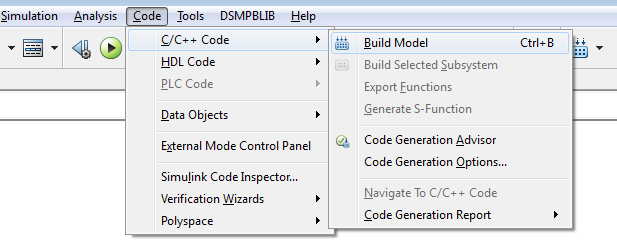
\includegraphics[width=0.7\textwidth]{Images/Ball and Bean/MatLab9.png}
        \caption{Generation of C code}
        \label{fig10}
    \end{figure}
    
    \begin{figure}[H]
        \centering
        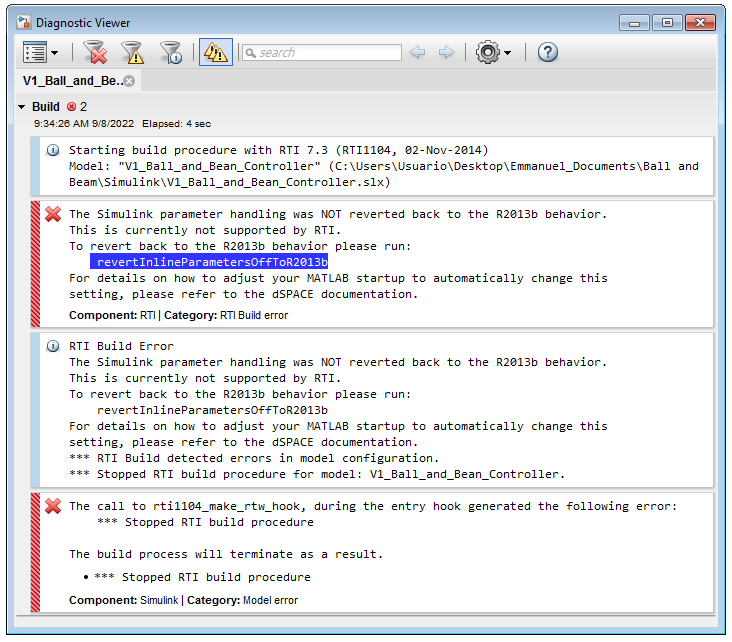
\includegraphics[width=0.7\textwidth]{Images/Ball and Bean/MatLab10.png}
        \caption{RTI Error message}
        \label{fig11}
    \end{figure}
    
    \begin{figure}[H]
        \centering
        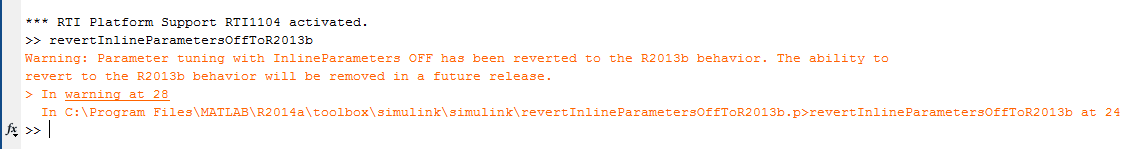
\includegraphics[width=0.7\textwidth]{Images/Ball and Bean/MatLab11.png}
        \caption{Command window of MATLAB after the correction of the error}
        \label{fig12}
    \end{figure}
    
    \begin{figure}[H]
        \centering
        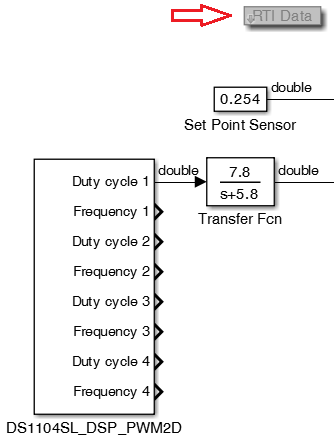
\includegraphics[width=0.5\textwidth]{Images/Ball and Bean/MatLab12.png}
        \caption{‘RTI Data’ symbol in the Simulink model}
        \label{fig13}
    \end{figure}
\end{enumerate}

\subsection{dSPACE Simulink blocks}

In Simulink, there is available a library of blocks related to the dSPACE board.
    
    \begin{figure}[H]
        \centering
        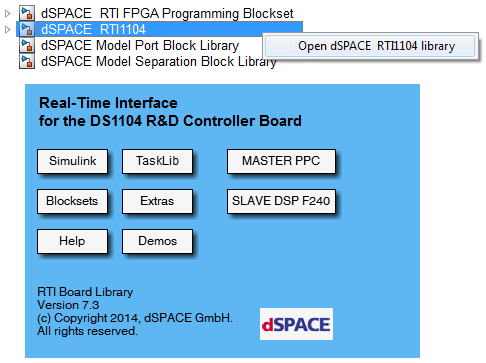
\includegraphics[width=0.7\textwidth]{Images/Ball and Bean/MatLab4.png}
        \caption{dSPACE libraries in Simulink.}
        \label{fig5}
    \end{figure}
By clicking on the SLAVE DSP F240 button, the window shown in figure \ref{fig14} be displayed.

     \begin{figure}[H]
        \centering
        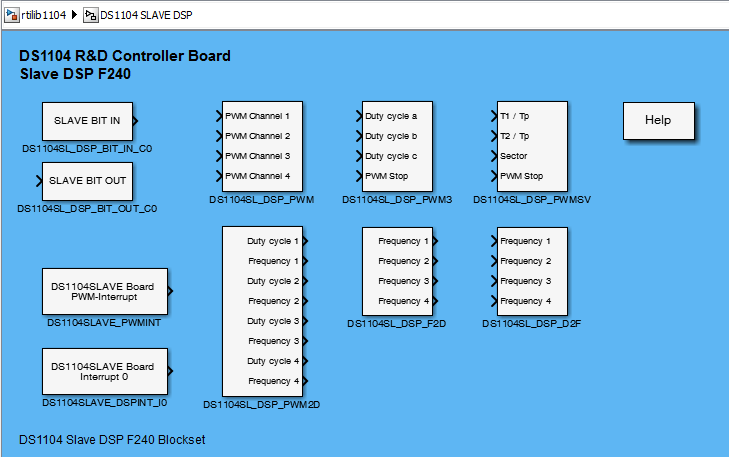
\includegraphics[width=0.7\textwidth]{Images/Ball and Bean/MatLab13.png}
        \caption{DS1104 Slave DSP F240 Blockset}
        \label{fig14}
    \end{figure}
Here you can find all the blocks related to the DS1104 slave DSP module.
For this project only two blocks will be needed:
\begin{enumerate}
    \item \textbf{DS1104SL\_DSP\_PWM}: for 1 phase PWM generation.
    \item \textbf{DS1104SL\_DSP\_PWM2D}: for sensor echo reading.
\end{enumerate}

\subsection{Basics of Slave DSP PWM Signal Generation}
The slave DSP of the DS1104 provides outputs for PWM signal generation. Each PWM pulse is centered around the middle of the corresponding PWM period (symmetric PWM generation mode) or in phase with the start of the period (asymmetric PWM generation mode).

\noindent \textbf{PWM signals}\par

PWM signal generation is crucial to many motor and motion control applications. PWM signals are pulse trains with fixed frequency and magnitude and variable pulse width. There is one pulse of fixed magnitude in every PWM period.

However, the width of the pulses changes from period to period according to a modulating signal. When a PWM signal is applied to the gate of a power transistor, it causes the turn-on/turn-off intervals of the transistor to change from one PWM period to another, according to the same modulating signal. The frequency of a PWM signal is usually much higher than that of the modulating signal, or the fundamental frequency, so that the energy delivered to the motor and its load depends mainly on the modulating signal.

\noindent \textbf{PWM period, duty cycle and resolution}\par

For PWM signals, you can specify the PWM period TP (= T$_high$+ T$_low$) in the range 200 ns … 819,2 ms. For 1-phase PWM signals, the PWM period TP applies to each of the four PWM output channels.

You can also specify the duty cycle. The following illustration shows how the duty cycle d (= T$_high$/ TP) is defined. The available duty cycle range is 0 … 1 (0 … 100 \%).

\begin{figure}[H]
    \centering
    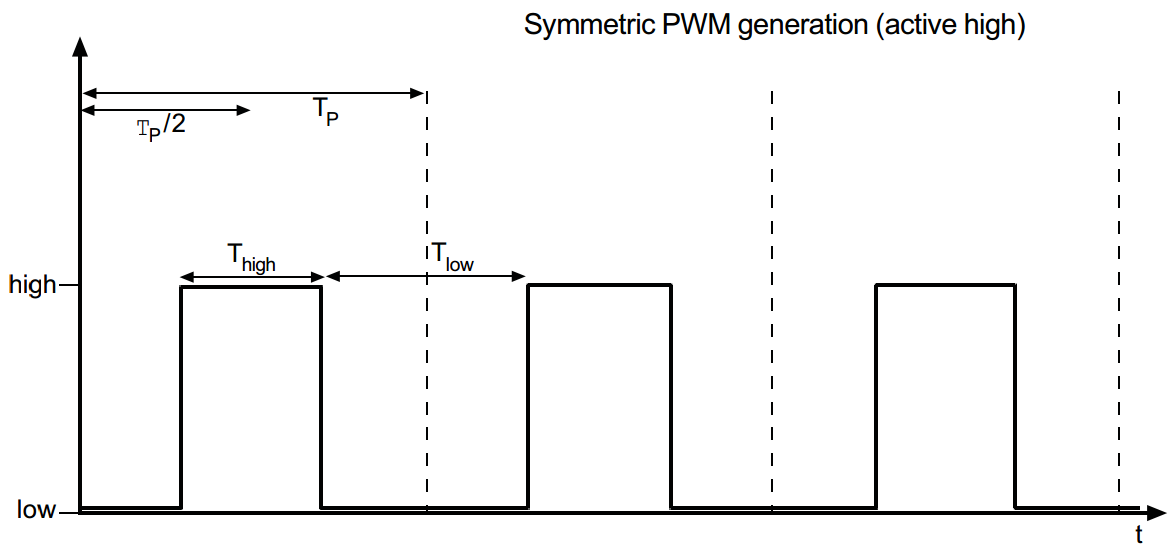
\includegraphics[width=\textwidth]{Images/Symmetric PWM generation.png}
    \caption{Symmetric PWM generation}
    %\label{Symmetric PWM generation}
\end{figure}

Depending on the selected PWM period, the following resolutions are given. They apply to symmetric PWM signals.

\begin{table}[H]
\centering
\begin{tabular}{|l|l|}
\hline
\rowcolor[HTML]{34CDF9} 
\textbf{Period T$_p$} & \textbf{Resolution} \\ \hline
\textless 6.4 ms   & 100 ns              \\
\textless 12.8 ms  & 200 ns              \\
\textless 25.6 ms  & 400 ns              \\
\textless 51.2 ms  & 800 ns              \\
\textless 102.4 ms & 1.6 $\mu$s              \\
\textless 204.8 ms & 3.2 $\mu$s              \\
\textless 409.6 ms & 6.4 $\mu$s              \\
\textless 819.2 ms & 12.8 $\mu$s             \\ \hline
\end{tabular}
\caption{Symmetric PWM resolution}
%\label{Symmetric PWM resolution}
\end{table}

\noindent \textbf{Asymmetric PWM mode}

As an alternative to the symmetric PWM generation mode, you can also let each PWM pulse start at the beginning of the corresponding PWM period (asymmetric PWM mode). Switching between symmetric and asymmetric PWM mode applies to all of the four 1-phase PWM output channels. The following illustration shows two active high symmetric and asymmetric 1-phase PWM signals.
\begin{figure}[H]
    \centering
    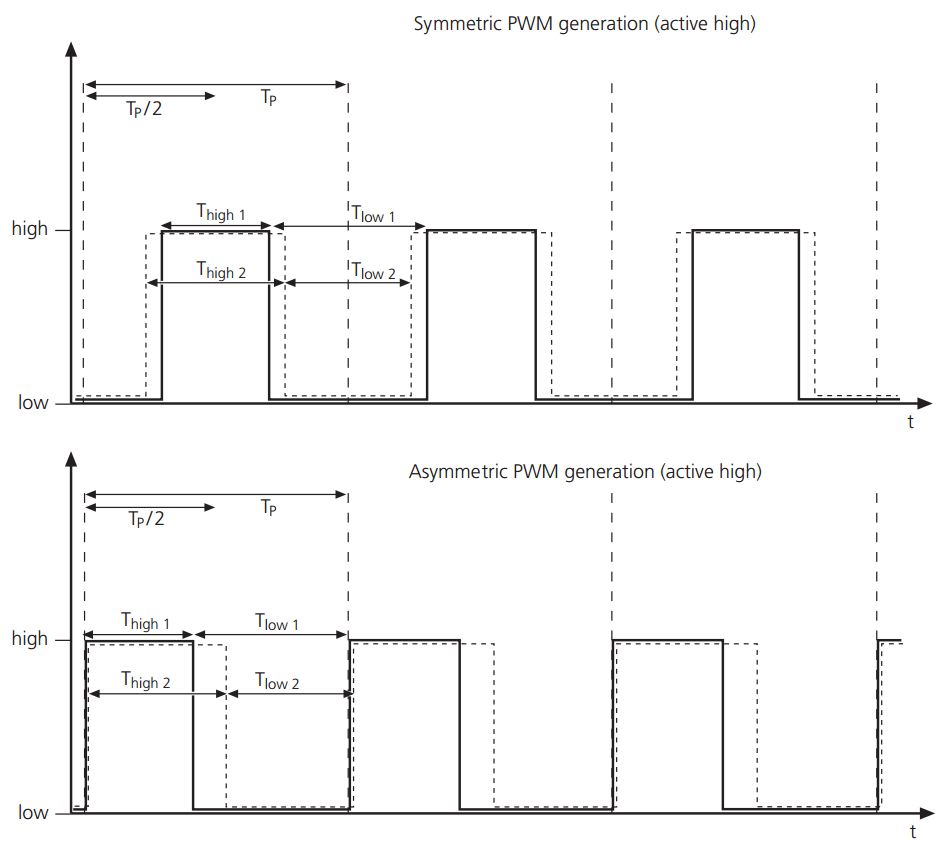
\includegraphics[width=0.8\textwidth]{Images/Symmetric and asymmetric PWM generation.png}
    \caption{Symmetric and asymmetric PWM generation}
    %\label{Symmetric and asymmetric PWM generation}
\end{figure}

\noindent \textbf{PWM period and resolution in asymmetric mode}\par

In the asymmetric mode, the PWM period T$_P$ must be in the range 200 ns … 409,6 ms. Depending on the period, the following resolutions are given:

\begin{table}[H]
\centering
\begin{tabular}{|l|l|}
\hline
\rowcolor[HTML]{34CDF9} 
\textbf{Period T$_p$} & \textbf{Resolution} \\ \hline
\textless 3.2 ms   & 50 ns              \\
\textless 6.4 ms   & 100 ns              \\
\textless 12.8 ms  & 200 ns              \\
\textless 25.6 ms  & 400 ns              \\
\textless 51.2 ms  & 800 ns              \\
\textless 102.4 ms & 1.6 $\mu$s              \\
\textless 204.8 ms & 3.2 $\mu$s              \\
\textless 409.6 ms & 6.4 $\mu$s              \\ \hline
\end{tabular}
\caption{Asymmetric PWM resolution}
%\label{Asymmetric PWM resolution}
\end{table}
\noindent \textit{Due to quantization effects, you will encounter considerable deviations between the desired PWM period T$_P$ and the generated PWM period, especially for higher PWM frequencies.}

\noindent \textbf{PWM outputs}\par
The PWM outputs can be specified. The running PWM generation can be suspended and the corresponding channels can be set to a specified TTL level (high or low). Only the output of the PWM signal is disabled. Signal calculation is still running and if you enable PWM generation, the currently calculated signal is output, and not the defined initialization or termination value. The PWM outputs can be specified for the two simulation phases (RTI):
\begin{itemize}
    \item During the initialization phase, you can disable the PWM generation of selected channels and set each output (pair) to a defined TTL level (high or low). No signal is generated during the initialization.
    \item During run time, you can stop PWM generation and set the outputs to a defined TTL level (high or low). At any time you can resume in generating the PWM signal. If the simulation terminates the outputs can be set to defined TTL levels.
\end{itemize}

If the PWM stop feature is disabled, the normal initialization and termination routines are executed. That means the specified duty cycles for initialization and termination are used.

\subsection{1-Phase PWM Signal Generation - DS1104SL\_DSP\_PWM}

    \begin{figure}[H]
        \centering
        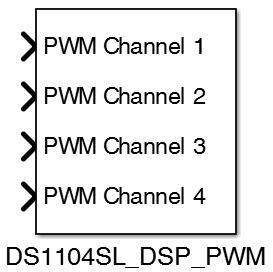
\includegraphics[width=0.35\textwidth]{Images/Ball and Bean/MatLab14.png}
        \caption{DS1104SL\_DSP\_PWM module in Simulink}
        \label{fig15}
    \end{figure}

\noindent \textbf{Purpose}\par
To generate standard PWM signals with variable duty cycles and enable PWM stop during run time.

\noindent \textbf{Description}\par 
For 1-phase PWM generation, a PWM stop can be specified to suspend PWM signal output during run time. The outputs of the channels are set to a defined TTL level. The dimensions of the inports are set to 2, which allows you to enter two values over the same port. This can be done via a Simulink MUX block, for example. Value 1 specifies the duty cycle and value 2 the PWM stop behavior. If you set value 2 to “0” a PWM signal is generated, “1” suspends signal generation and sets the output to the specified TTL level. If the PWM stop is disabled for a channel only the duty cycle can be input. Although you can disable the PWM stop feature for each channel during run time, you can specify whether you want to set the PWM output to a specified TTL level or to generate a signal during the initialation phase.

\noindent \textbf{I/O mapping}\par 

\begin{table}[H]
\begin{adjustbox}{width=1\textwidth}
\small
\begin{tabular}{|lllll|}
\hline
\rowcolor[HTML]{34CDF9} 
\multicolumn{1}{|l|}{\cellcolor[HTML]{34CDF9}\textbf{Signal}} &
  \multicolumn{3}{l|}{\cellcolor[HTML]{34CDF9}\textbf{Channel/Bit Numbers of Related RTI Blocks/RTLib Functions}} &
  {\cellcolor[HTML]{34CDF9}\textbf{I/O Pin on …}} \\ \cline{2-5} 
\rowcolor[HTML]{34CDF9} 
\multicolumn{1}{|l|}{\cellcolor[HTML]{34CDF9}\textbf{}} &
  \multicolumn{1}{l|}{\cellcolor[HTML]{34CDF9}\textbf{Related RTI Block(s)}} &
  \multicolumn{1}{l|}{\cellcolor[HTML]{34CDF9}\textbf{Ch/Bit (RTI)}} &
  \multicolumn{1}{l|}{\cellcolor[HTML]{34CDF9}\textbf{Ch/Bit (RTILib)}} &
  \textbf{D-SUB 37} \\ \hline
\multicolumn{5}{|l|}{\textbf{1‑Phase PWM Signal Generation (PWM)}} \\ \hline
\multicolumn{5}{|l|}{\tabitem TTL output voltage range} \\
\multicolumn{5}{|l|}{\tabitem Output current range: ±13 mA} \\
\multicolumn{1}{|l|}{ST2PWM} &
  \multicolumn{1}{l|}{DS1104SL\_DSP\_PWM} &
  \multicolumn{1}{l|}{Channel 1} &
  \multicolumn{1}{l|}{Channel 1} &
  5 \\
\multicolumn{1}{|l|}{SPWM7} &
  \multicolumn{1}{l|}{} &
  \multicolumn{1}{l|}{Channel 2} &
  \multicolumn{1}{l|}{Channel 2} &
  10 \\
\multicolumn{1}{|l|}{SPWM8} &
  \multicolumn{1}{l|}{} &
  \multicolumn{1}{l|}{Channel 3} &
  \multicolumn{1}{l|}{Channel 3} &
  29 \\
\multicolumn{1}{|l|}{SPWM9} &
  \multicolumn{1}{l|}{} &
  \multicolumn{1}{l|}{Channel 4} &
  \multicolumn{1}{l|}{Channel 4} &
  11 \\ \hline
\end{tabular}
\end{adjustbox}
\caption{Slave DSP 1-phase PWM Signal}
\label{Slave DSP 1-phase PWM Signal}
\end{table}

\noindent \textbf{I/O characteristics}\par

\begin{table}[H]
\begin{adjustbox}{width=1\textwidth}
\begin{tabular}{|l|l|l|l|l|}
\hline
\rowcolor[HTML]{34CDF9} 
\textbf{Simulink Inport} & \textbf{Input}   & \textbf{Value} & \textbf{Data Type} & \textbf{Meaning}                                 \\ \hline
PWM Channel 1 … 4        & Duty cycle 1 … 4 & 0 ... 1        & Double             & Duty cycle of the PWM signal for channel 1 ... 4 \\
                         & PWM Stop 1 … 4   & 0 ... 1        & Boolean            & Enables PWM stop for channel 1 … 4:              \\
 &  &  &  & \tabitem Value 1 stops PWM generation   \\
 &  &  &  & \tabitem Value 0 resumes PWM generation \\ \hline
\end{tabular}
\end{adjustbox}
\caption{1-phase PWM Signal Simulink data types}
\label{1-phase PWM Signal Simulink data types}
\end{table}

\subsubsection{Simulink implementation}
The DS1104SL\_DSP\_PWM inputs PWM Channel 1 ... 3 were used and channel 4 was disabled.
\begin{itemize}
    \item \textbf{PWM Channel 1}, is used for pulse generation for triggering the HC-SR04 ultrasonic sensor.
    \item \textbf{PWM Channel 2}, is used to command the servo motor linked to the sensor and the ball guide.
    \item \textbf{PWM channel 3}, is used to lock the two servo motors of the base. Just to make sure that nothing will move unintentionally.
    \item \textbf{PWM channel 4}, disabled.
\end{itemize}
The block was configured to operate at \textcolor{red}{\textbf{50 Hz}} in \textcolor{red}{\textbf{asymmetric mode}}. All other parameters were left at their default values.
Like mentioned above, all four inputs were multiplexed with a \textcolor{red}{\textbf{STOP bit}} to provide the start/stop option.
    \begin{figure}[H]
        \centering
        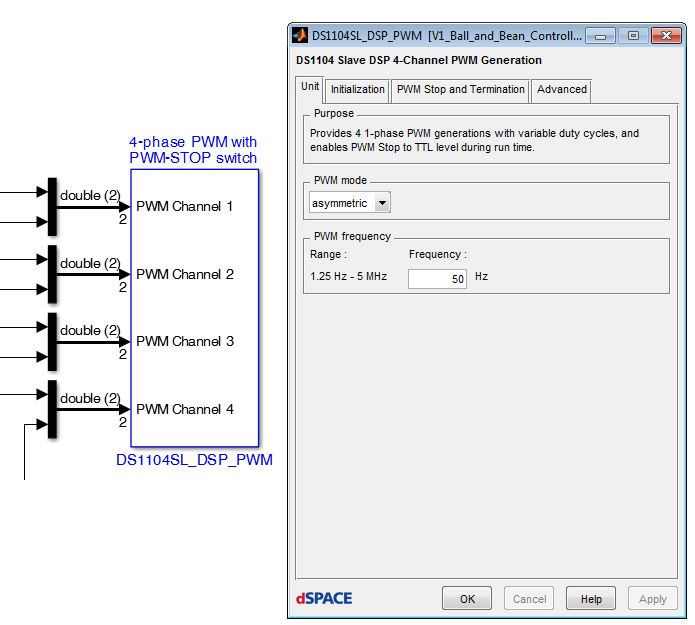
\includegraphics[width=0.7\textwidth]{Images/Ball and Bean/MatLab17.png}
        \caption{PWM module in Simulink}
        \label{fig18}
    \end{figure}

\subsection{1-Phase PWM Signal Measurement - DS1104SL\_DSP\_PWM2D}
In this case the DS1104SL\_DSP\_PWM2D block is used.\par
It can measure the duty cycles and the frequencies from up to 4 independent channels used for PWM-type signals.\\
The reason for its use is because the HC-SR04 returns a high pulse proportional to the duration of the echo of the sound emitted by the sensor actuator.\par
The measurement algorithm used is accurate if the PWM period starts
with the falling or rising edge of the corresponding PWM signal so, the PWM module must be in \textcolor{red}{\textbf{asymmetric mode}}.\par
As only one signal will be measured, channel 1 is used to measure its duty cycle.

\begin{table}[H]
\begin{adjustbox}{width=1\textwidth}
\small
\begin{tabular}{|lllll|}
\hline
\rowcolor[HTML]{34CDF9} 
\multicolumn{1}{|l|}{\cellcolor[HTML]{34CDF9}\textbf{Signal}} &
  \multicolumn{3}{l|}{\cellcolor[HTML]{34CDF9}\textbf{Channel/Bit Numbers of Related RTI Blocks/RTLib Functions}} &
  {\cellcolor[HTML]{34CDF9}\textbf{I/O Pin on …}} \\ \cline{2-5} 
\rowcolor[HTML]{34CDF9} 
\multicolumn{1}{|l|}{\cellcolor[HTML]{34CDF9}\textbf{}} &
  \multicolumn{1}{l|}{\cellcolor[HTML]{34CDF9}\textbf{Related RTI Block(s)}} &
  \multicolumn{1}{l|}{\cellcolor[HTML]{34CDF9}\textbf{Ch/Bit (RTI)}} &
  \multicolumn{1}{l|}{\cellcolor[HTML]{34CDF9}\textbf{Ch/Bit (RTILib)}} &
  \textbf{D-SUB 37} \\ \hline
\multicolumn{5}{|l|}{\textbf{Slave DSP PWM Signal Measurement (PWM2D)}} \\ \hline
\multicolumn{5}{|l|}{\tabitem TTL input voltage range 0 - 5V} \\
\multicolumn{5}{|l|}{\tabitem Input current: 500 $\mu$A} \\
\multicolumn{1}{|l|}{SCAP1} &
  \multicolumn{1}{l|}{DS1104SL\_DSP\_PWM2D} &
  \multicolumn{1}{l|}{Channel 1} &
  \multicolumn{1}{l|}{Channel 1} &
  2 \\
\multicolumn{1}{|l|}{SCAP2} &
  \multicolumn{1}{l|}{} &
  \multicolumn{1}{l|}{Channel 2} &
  \multicolumn{1}{l|}{Channel 2} &
  21 \\
\multicolumn{1}{|l|}{SCAP3} &
  \multicolumn{1}{l|}{} &
  \multicolumn{1}{l|}{Channel 3} &
  \multicolumn{1}{l|}{Channel 3} &
  3 \\
\multicolumn{1}{|l|}{SCAP4} &
  \multicolumn{1}{l|}{} &
  \multicolumn{1}{l|}{Channel 4} &
  \multicolumn{1}{l|}{Channel 4} &
  22 \\ \hline
\end{tabular}
\end{adjustbox}
\caption{Signal mapping of Slave DSP PWM Signal Measurement (PWM2D)}
\label{Signal mapping of Slave DSP PWM Signal Measurement (PWM2D)}
\end{table}
    \begin{figure}[H]
        \centering
        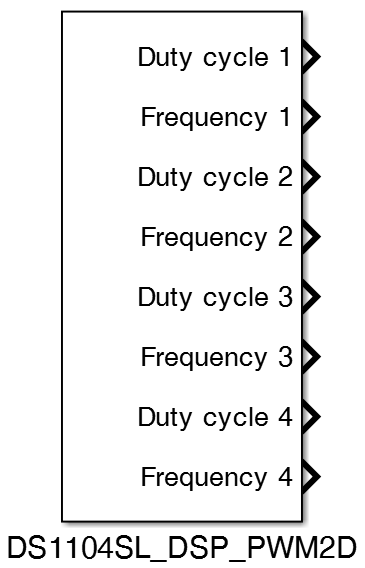
\includegraphics[width=0.4\textwidth]{Images/Ball and Bean/MatLab15.png}
        \caption{Measurement module in Simulink}
        \label{fig19}
    \end{figure}

\newpage

\subsection{Basic Operation and Timing of the HC-SRO4 Ultrasonic Sensor}

    \begin{figure}[H]
        \centering
        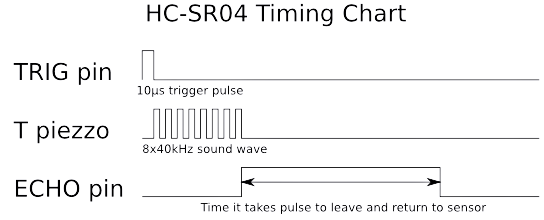
\includegraphics[width=0.6\textwidth]{Images/Ball and Bean/HC-SR04-Timing.png}
        \caption{HC-SR04 Timing chart}
        \label{fig20}
    \end{figure}
    \begin{enumerate}
        \item Make "Trig" (pin 2) on the sensor high for 10µs. This initiates a sensor cycle.
        \item 8x40kHz pulses will be sent from the "T" transmitting piezzo transducer of the sensor, after which time the "Echo" pin on the sensor will go from low to high.
        \item The 40kHz sound wave will bounce off the nearest object and return to the sensor.
        \item When the sensor detects the reflected sound wave, the the Echo pin will go low again.
        \item The distance between the sensor and the detected object can be calculated based on the length of time the Echo pin is high.
        \item If no object is detected, the Echo pin will stay high for 38ms and then go low.
    \end{enumerate}
    
\subsection{Basic Operation and Timing of Futaba S3003 Servomotor}
    \begin{figure}[H]
        \centering
        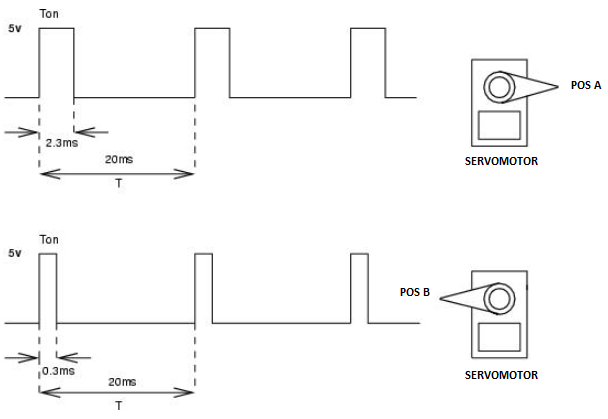
\includegraphics[width=0.5\textwidth]{Images/Ball and Bean/Servo2.png}
        \caption{Servomotor Timing chart}
        \label{fig21}
    \end{figure}
To position the servo, a periodic signal of 50Hz (20ms period) must be applied. The width of the pulse determines the servo position. If the width is 2.3ms, the servo is positioned at one end and if the width is 0.3ms it is positioned at the opposite end. Any other width between 0.3 and 2.3ms places the servo in a position between one end and the other. For example, if we want it to be positioned exactly in the center, we apply a width of 1.3ms.

When the signal is no longer sent, the servo enters an idle state, and can therefore be moved by hand. As long as the signal is applied, it will remain fixed in its position, forcing it to stay there.

\subsection{Finding the limits of the servomotor - Simulink example model}

Simulink has the simplicity of block programming and the programmer must have the skills to realize a simple, efficient and robust control system.

You must know how your servo motor operate and especially its limits. You can build a simple model in Simulink and find these limits with ControlDesk. Not all motors are the same and to be accurate, this is a necessary step.

For this example a \textit{20ms} period will be set, that is the typical value for this type of servomotors (this value also change whit the servomotor model).
    \begin{figure}[H]
        \centering
        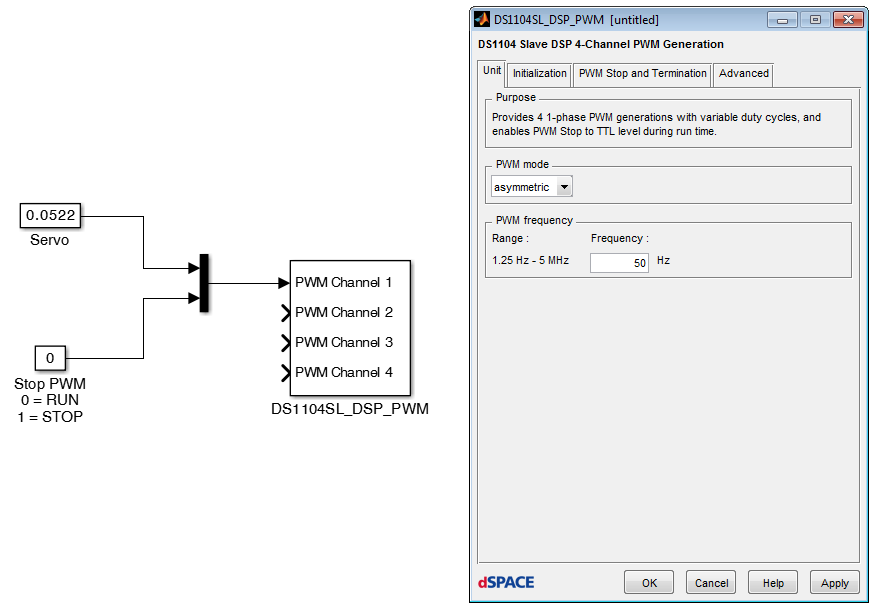
\includegraphics[width=0.6\textwidth]{Images/Ball and Bean/PWM_Example.png}
        \caption{Simulink servomotor test}
        \label{fig22}
    \end{figure}
You must now follow the compilation steps mentioned in the first section in order to work with ControDesk. After compilation process, the RTI Data symbol will appear.
       
     \begin{figure}[H]
        \centering
        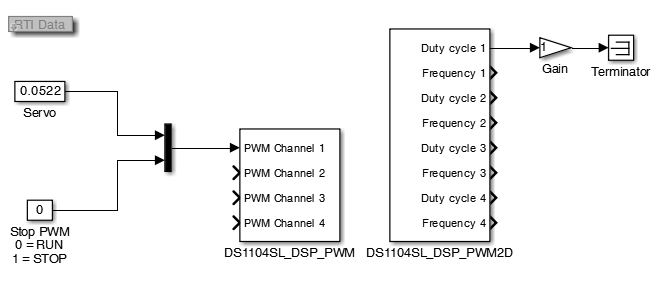
\includegraphics[width=0.8\textwidth]{Images/Ball and Bean/PWMExampleSimulink.png}
        \caption{Simulink model - servomotor test}
        \label{fig37}
    \end{figure}
    
With this model you will be able to test your servomotors to know their characteristics and operating limits.\par
Remember that most servomotors operate between 0,3 and 2,3 ms pulse width for their entire range of motion.

\subsection{ControlDesk interface}

\subsubsection{Creating a ControDesk project}
\begin{enumerate}
    \item Open ControlDesk 5.3. The first thing to do is to create a new project. This is done in the ‘File’ tab, in the option ‘New’, and selecting ‘Create New Project and Experiment’, as seen in figure \ref{fig24}.
    \begin{figure}[H]
        \centering
        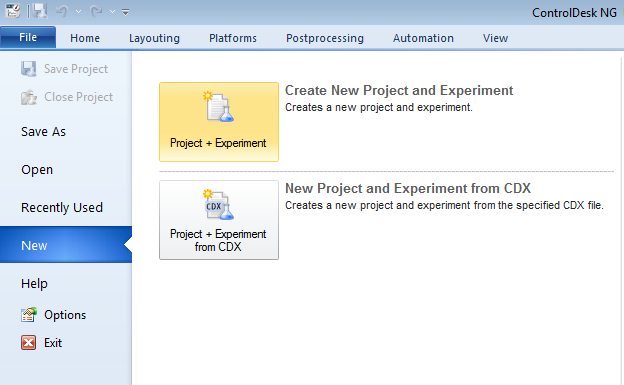
\includegraphics[width=0.5\textwidth]{Images/Ball and Bean/ControlDesk/CD1.png}
        \caption{Creation of a new project in ControlDesk}
        \label{fig24}
    \end{figure}
    \item A window will open. Select a name for the project and a root directory.
    \begin{figure}[H]
        \centering
        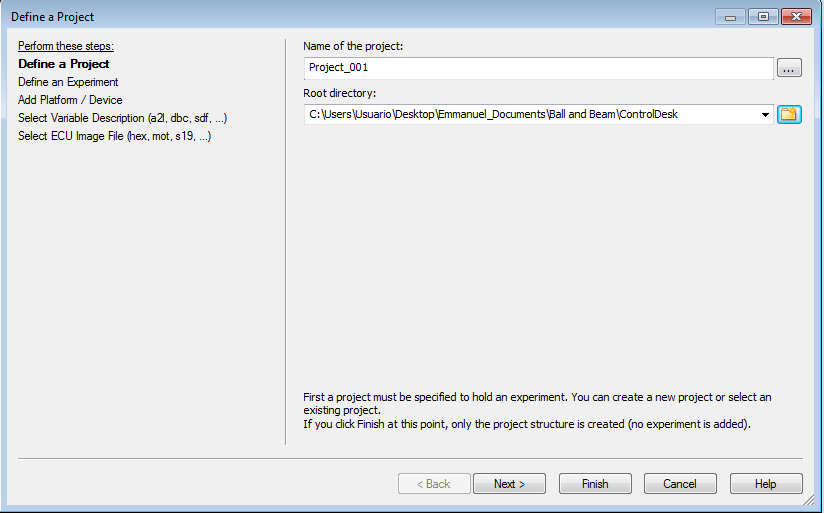
\includegraphics[width=0.5\textwidth]{Images/Ball and Bean/ControlDesk/CD2.png}
        \caption{Define a project}
        \label{fig25}
    \end{figure}
    \item The root directory must be in you project main folder. Just follow the steps in figure \ref{fig26}. 
    \begin{figure}[H]
        \centering
        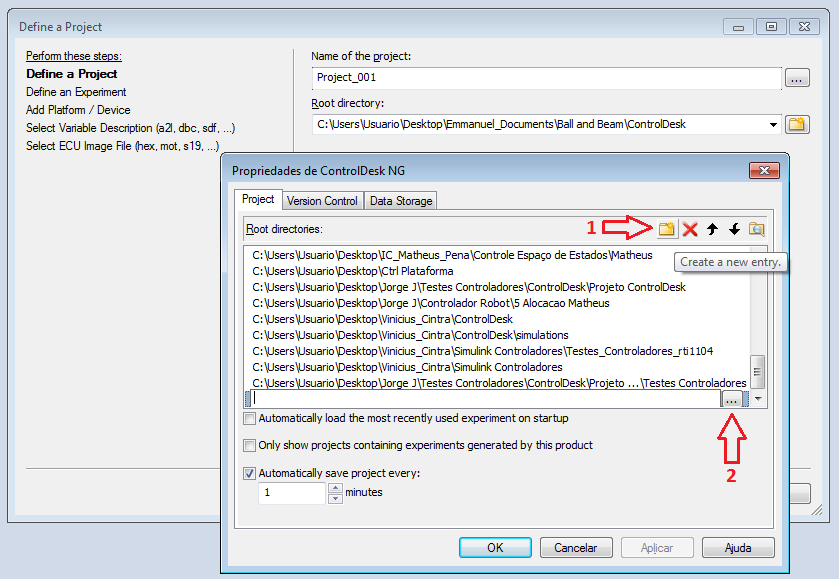
\includegraphics[width=0.5\textwidth]{Images/Ball and Bean/ControlDesk/CD3.png}
        \caption{Root directory}
        \label{fig26}
    \end{figure}
    \item After pressing ‘Next’, the user must select the controller board which is being used which, in this case, is the DS1104, as seen in figure \ref{fig27}.
    \begin{figure}[H]
        \centering
        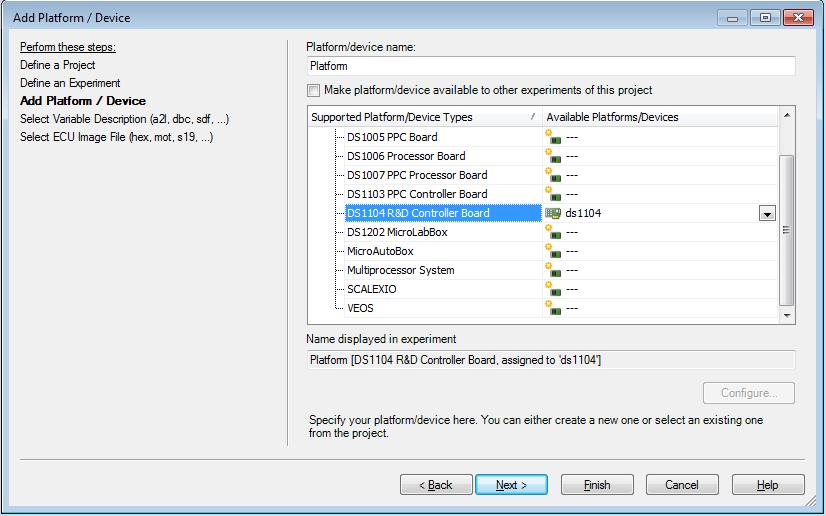
\includegraphics[width=0.5\textwidth]{Images/Ball and Bean/ControlDesk/CD4.png}
        \caption{Add plataform / Device}
        \label{fig27}
    \end{figure}
    \item To associate the variables from the Simulink model with ControlDesk, the \textcolor{red}{\textbf{.sdf}} file generated during the compilation of the code done previously must be imported by pressing the button ‘Import from file...’, and selecting it, as seen in figure \ref{fig28}. After this is done, press ‘Finish’.
    \begin{figure}[H]
        \centering
        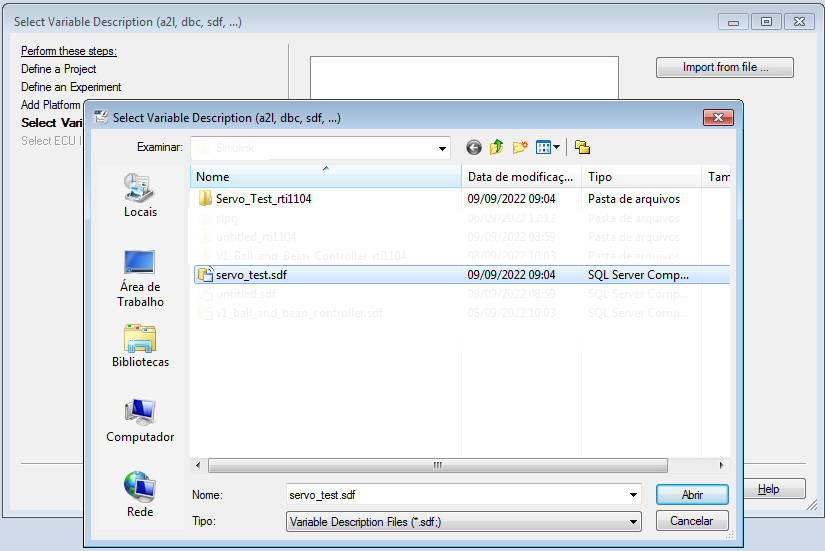
\includegraphics[width=0.5\textwidth]{Images/Ball and Bean/ControlDesk/CD5.png}
        \caption{Select variable description}
        \label{fig28}
    \end{figure}
    \item The software offers a variety of tools and options. The ones of interest are highlighted with colors in figure \ref{fig29}, are described below:
    \begin{itemize}
        \item Yellow area: corresponds to the lead toolbar.
        \item Red area: corresponds to the work area. In this zone, a variety of instruments like indicators, graphs, and numeric inputs can be placed, to create a ‘Layout’, which acts as a interface between the user and the controller.
        \item Blue area: the instrument selector shows all the instruments available. If this list does not appear at the moment the project is created, it can be activated in the menu ‘Layouting’, and selecting ‘Insert Instrument’.
        \item Green area: shows the variables associated with the imported Simulink model, or models. The instruments in the layout can be associated to variables of the Simulink model.
    \end{itemize}
    \begin{figure}[H]
        \centering
        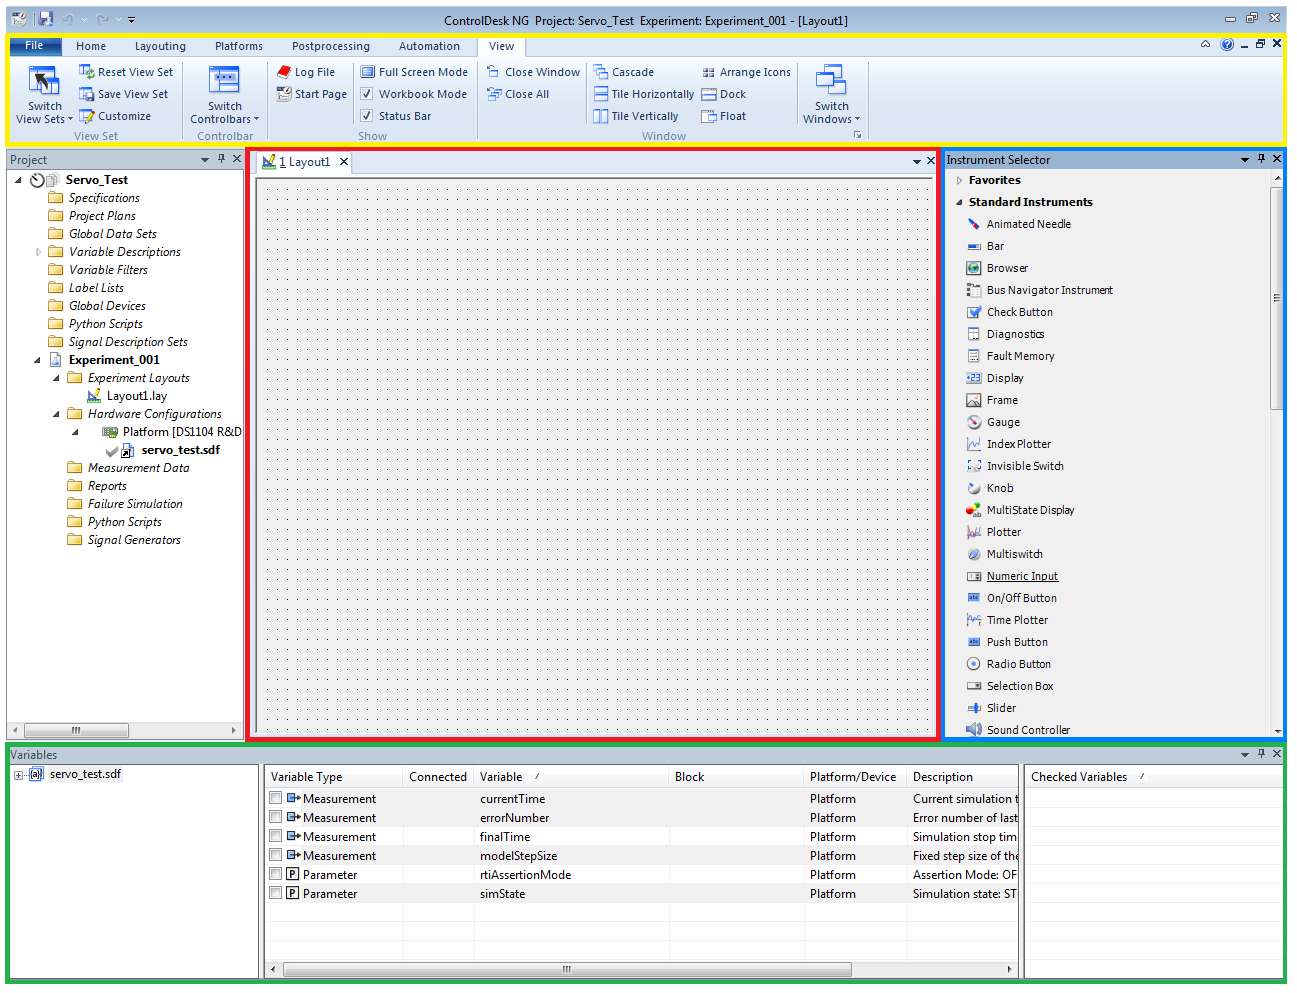
\includegraphics[width=0.8\textwidth]{Images/Ball and Bean/ControlDesk/CD6.png}
        \caption{ControlDesk window}
        \label{fig29}
    \end{figure}
    
\end{enumerate}


\subsubsection{Data recording}

\begin{enumerate}
    \item To be able to work with historical data of the variables, it is necessary to record their behavior during a real time experiment, and export them to a file. To analyze the data in MATLAB, a file can be generated with the recorder tool of ControlDesk. To display the ‘Measurement Configuration’ bar, go to the tab ‘View’, click on ‘Switch Controlbars’ and select ‘Measurement Configuration’, as seen in figure \ref{fig30}
    \begin{figure}[H]
        \centering
        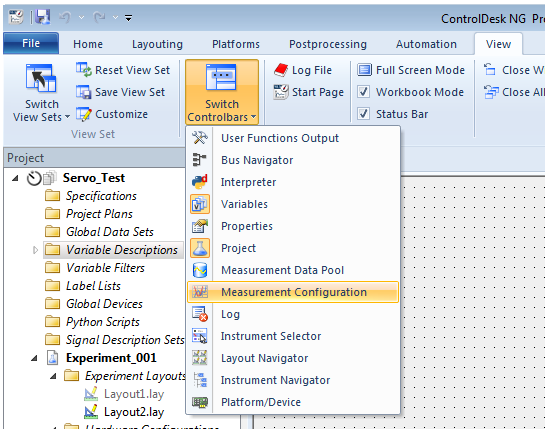
\includegraphics[width=0.8\textwidth]{Images/Ball and Bean/ControlDesk/CD7.png}
        \caption{Activation of the recording tool bar}
        \label{fig30}
    \end{figure}
    \item In the ‘Measurement Configuration’ bar one can find the ‘Recorders’. ControlDesk records the variables shown in the ‘Plotters’ of the layout by default, so the ‘Recorder 1’ corresponds to the actives plotters. To record another variable, one can drag and drop a variable from the ‘Variables’ bar to a existing recorder, or create one by right-clicking on ‘Recorders’, and selecting ‘Create New Recorder’.

    \item Right-click on ‘Recorder 1’ and select ‘Properties’ to open the dialog seen in figure \ref{fig31}. Select ‘Automatic export’ to automatically create a file with the recording of the variable, and select a name for the file, the folder where the file will be generated, and the file type. To be able to work the data in MATLAB select ‘MATLAB file (*.mat)’. Also, the name of the recorder can be changed
    \begin{figure}[H]
        \centering
        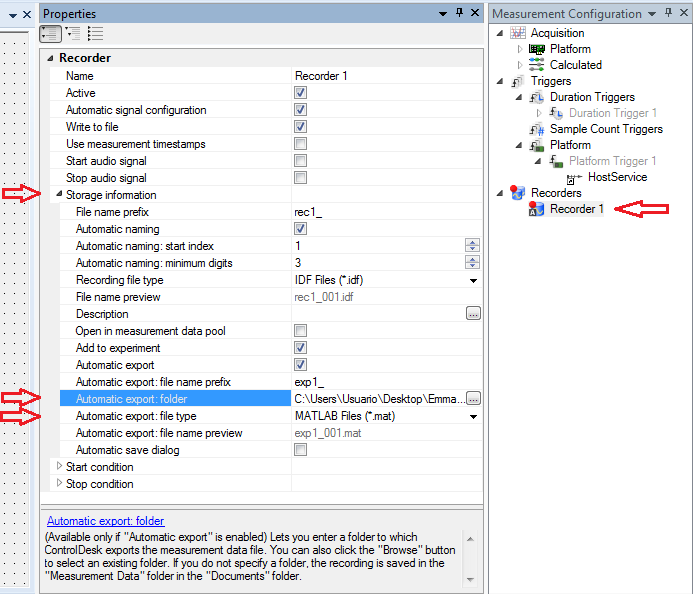
\includegraphics[width=0.8\textwidth]{Images/Ball and Bean/ControlDesk/CD8.png}
        \caption{Properties of the recorder}
        \label{fig31}
    \end{figure}

    \item To record the data, in the ‘Home’ tab, select ‘Start Immediate’ when the experiment is running, or any other time to initiate the experiment and record from the beginning. Also, the recording can be set to start automatically in response to a variable value or a logical expression, by selecting ‘Trigger Rules’.
    \begin{figure}[H]
        \centering
        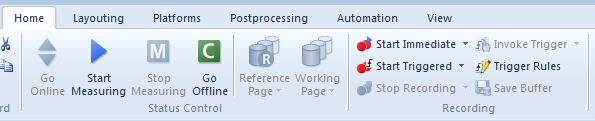
\includegraphics[width=0.8\textwidth]{Images/Ball and Bean/ControlDesk/CD9.png}
        \caption{Start recording}
        \label{fig32}
    \end{figure}
\end{enumerate}

\subsubsection{Layout interface}
The layout area corresponds to the zone were a variety of instruments like indicators, graphs, and numeric inputs can be placed, to create a ‘Layout’, which acts as a interface between the user and the controller.
For this example we only need a few elements:
\begin{enumerate}
    \item Numeric inputs: To work with the servo motor PWM and to START/STOP the PWM output.
    \item Numeric display: To visualize the value of the generated PWM.
    \item Time plotter: To visualize the value of the generated PWM over the time.
\end{enumerate}
To place components 1, 2 and 3 in the layout area, you have to drag and drop the corresponding variables from the \textbf{variables area} and then associate them with the desired instrument.
    \begin{figure}[H]
        \centering
        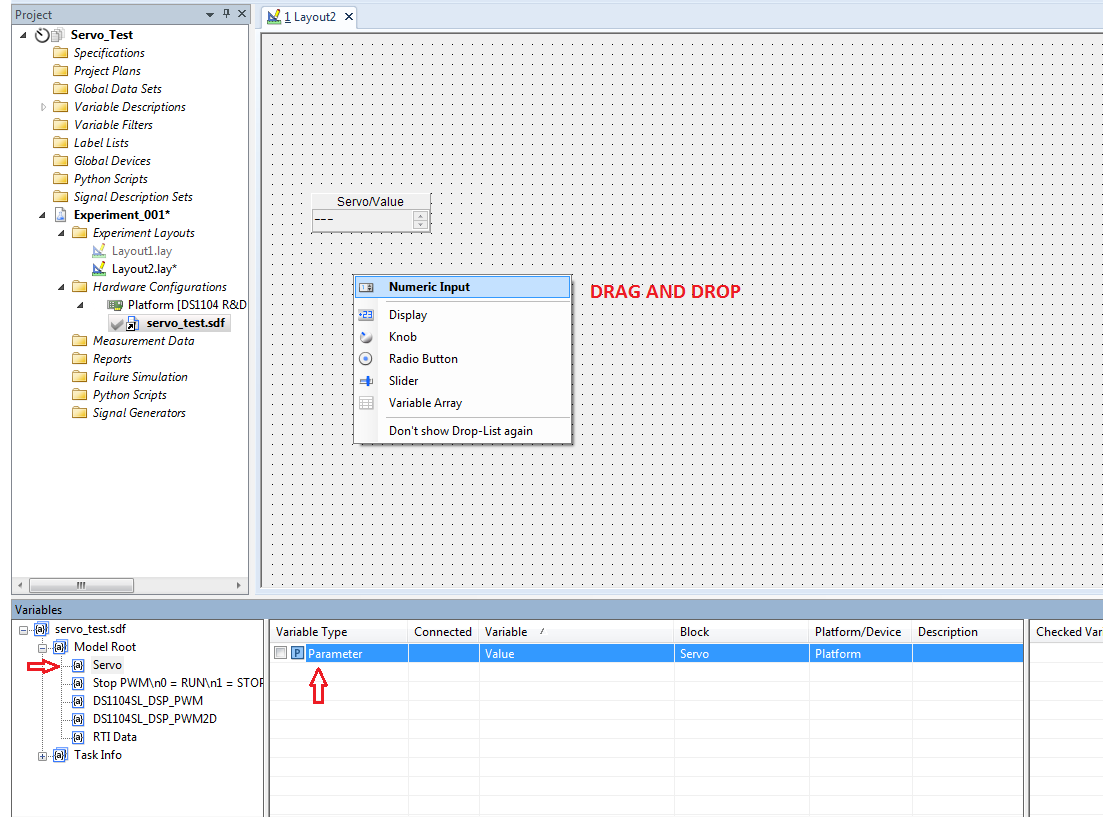
\includegraphics[width=0.8\textwidth]{Images/Ball and Bean/ControlDesk/CD10.png}
        \caption{Servo numeric input}
        \label{fig33}
    \end{figure}
    \begin{figure}[H]
        \centering
        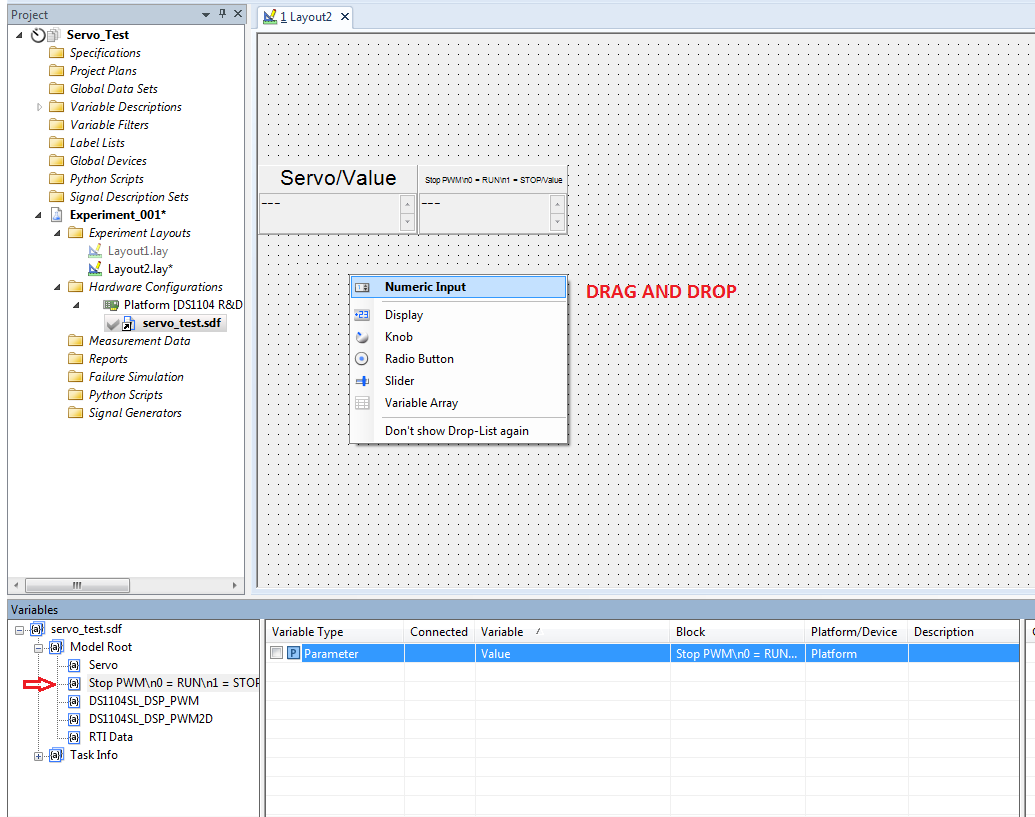
\includegraphics[width=0.8\textwidth]{Images/Ball and Bean/ControlDesk/CD11.png}
        \caption{START/STOP numeric input}
        \label{fig34}
    \end{figure}
    \begin{figure}[H]
        \centering
        \includegraphics[width=0.8\textwidth]{Images/Ball and Bean/ControlDesk/CD12.png}
        \caption{PWM numeric display}
        \label{fig35}
    \end{figure}
    \begin{figure}[H]
        \centering
        \includegraphics[width=0.8\textwidth]{Images/Ball and Bean/ControlDesk/CD13.png}
        \caption{Adding plotter linked to PWM duty cycle}
        \label{fig36}
    \end{figure}
With these items, you can now press the \textcolor{green}{\textbf{Go Online}} and \textcolor{blue}{\textbf{Start Measuring}} buttons to test the experiment.

\newpage

\section{Ball and beam software implementation}
The objective of this project is the practical implementation of a ball and beam system using the dSPACE digital control system with a servomotor, as actuator, and an ultrasonic sensor, as an element to measure error. 
Using the DS1104 Slave DSP F240 Blockset and the above mentioned blocks will help in these tasks.\par
\section{KiCAD}

\section{Ball and beam hardware implementation}



%%%%%%%%%%%%%%%%%%%%%%%%%%%%%%%%%%%%%%%%%%%%%%%%%%%%%%%%%%%%%%%%%%%%%

\newpage
\printbibliography[
heading=bibintoc,
title={References}
]

\newpage
\appendix

\includepdf[pages=-,pagecommand=\thispagestyle{plain}]{Datasheets/Datasheet - futaba S3003.pdf}

\includepdf[pages=-,pagecommand=\thispagestyle{plain}]{Datasheets/Datasheet - HC-SR04.pdf}

\end{document}
